\documentclass{article}
\usepackage{amsthm}
\usepackage[utf8x]{inputenc}
\usepackage[usenames,dvipsnames]{color}
\author{Simone Gasperoni}
\theoremstyle{plain}
\newtheorem{thm}{Teorema}[] 
\theoremstyle{definition}
\newtheorem{defn}[]{Definizione} % definition numbers are dependent on theorem numbers
\newtheorem{exmp}[thm]{Example} % same for example numbers
\usepackage{dirtytalk}
\usepackage{graphicx}
\usepackage{listings}
\usepackage{amsmath}
\usepackage{color}
\usepackage{hyperref}
\definecolor{dkgreen}{rgb}{0,0.6,0}
\definecolor{gray}{rgb}{0.5,0.5,0.5}
\definecolor{mauve}{rgb}{0.58,0,0.82}

\lstset{frame=tb,
	language=python,
	aboveskip=3mm,
	belowskip=3mm,
	showstringspaces=false,
	columns=flexible,
	basicstyle={\small\ttfamily},
	numbers=none,
	numberstyle=\tiny\color{gray},
	keywordstyle=\color{blue},
	commentstyle=\color{dkgreen},
	stringstyle=\color{mauve},
	breaklines=true,
	breakatwhitespace=true,
	tabsize=3
}

\author{Simone Gasperoni}
\title{Categorizzazione degli open-data italiani sul profilo europeo dei metadati DCAT-AP}

\begin{document}

\begin{titlepage}
\begin{center}

\textsc{Laurea magistrale in Ingegneria informatica (D.M. 270)}\\[0.5cm]
\textsc{Università degli studi di Roma Tre}\\[0.5cm]

\hrulefill

{ \huge \bfseries Categorizzazione degli open-data italiani sul profilo europeo dei metadati DCAT-AP \\[0.4cm] }
\textsc{\Large Simone Gasperoni}\\[0.5cm]
\vfill
\LaTeX


Roma, Italia
\end{center}
\end{titlepage}


\tableofcontents


\newpage

\topskip0pt
\vspace*{\fill}
\textit{
\\
\\
\say{Data is a precious thing and will last longer than the systems themselves.}} 
\\
Tim Berners-Lee
\\
\\
\textit{
\say{Who has the data has the power.}}
\\
Tim O'Reilly 
\vspace*{\fill}
\newpage

\newpage
\section{Introduzione}
\newpage
\section{Contesto}
\subsubsection{Semantic web}
Al giorno d'oggi il web ha cambiato sia il modo di comunicare con le persone sia il modo di utilizzare il computer. In passato, l'elaboratore veniva utilizzato espressamente solo per l'elaborazione di calcoli, oggi, invece, incorpora strumenti per processare informazioni testuali e multimediali. Gli utenti del web usano il computer soprattutto per effettuare ricerche di informazioni di carattere generale (come la ricerca di informazioni di altre persone), per entrare in contatto con altre persone, per consultare cataloghi, e per ordinare prodotti di negozi on-line, ... Tutte queste attività sono rese possibili grazie all'utilizzo di strumenti particolari quali i motori di ricerca. 
\\
\\
Essi hanno avuto un grande successo e hanno contribuito al miglioramento del web, tuttavia, basandosi su un matching tra le parole chiave, hanno bisogno dell'intervento umano per interpretare e combinare i risultati che propongono. Questo è dovuto al fatto che i risultati delle ricerche non sono facilmente accessibili da altri strumenti e quindi il significato del contenuto non è accessibile alla macchina. 
\\
\\
Il web semantico si pone nella prospettiva di andare oltre questo tipo di limitazioni del web, si vuole infatti rappresentare il web in un modo diverso, utilizzando tecniche intelligenti affinché anche le macchine possano interpretare le informazioni.
\\
\\
Nel 2001, nel pieno della pur continua espansione del web e dei suoi molteplici utilizzi Tim Berners-Lee, James Hendler, e Ora Lassila pubblicavano un articolo che sarebbe diventato una pietra miliare. In esso l'inventore del web, insieme ai suoi co-autori lanciavano il web semantico definendolo come una \say{estensione del web attuale, in cui all'informazione è dato un ben determinato significato, facilitando la cooperazione tra i computer e le persone}. In estrema sintesi, la visione espressa era di un web in cui l'enfasi si sposta dai documenti - e dalla relativa interpretazione da parte degli umani - ai dati e al loro significato e interpretazione da parte degli elaboratori.
\\ 
\\
Ad onor del vero già da qualche anno diversi studi e progetti, sia in Europa che negli USA, indicavano le opportunità, quasi la necessità, del passaggio ad un web in cui oltre che il puro testo ci fosse una qualche forma di struttura atta a facilitare la comprensione da parte delle macchine del contenuto delle pagine web e una maggiore interoperabilità. 
\\
\\
L'appoggio e il sostegno del creatore del web e direttore del W3C rappresentavano però un evidente viatico e sprone a reinventare il web, passando da un web di documenti collegati tra di loro ad uno di dati interconnessi.
\footnotemark
\footnotetext{Di Noia, De Virgilio, Di Sciascio, Donini, Semantic Web: Tra ontologie e Open Data, Apogeo, 2013}
\\
\\
Il semantic web è l'evoluzione del vecchio web dove si associa ad ogni documento un'etichettatura intelligente (metadati), al fine di correlare una semantica ai dati, e le informazioni possono essere collegate ed integrate tra loro. Grazie al web semantico, dunque, è possibile effettuare operazione specialistiche e ricerche altamente più precise.

\subsection{Linked Open Data}
Il W3 Consortium definisce il web semantico: \say{web dei dati}, proprio perché al suo interno ha un elevato numero di documenti ed informazioni che sono accessibili a tutti liberamente (open-data). Affinché i risultati ottenuti dalle attività di recupero delle informazioni siano di reale utilità per l'utente risulterebbe di grande vantaggio che i dati fossero proposti all'utente in forma aggregata, anziché isolata.
\\
\\
Vi è infatti l'esigenza di esplicitare i collegamenti tra le informazioni, anche se questi sono di differente formato e provengono da fonti eterogenee. Per realizzare il collegamento tra i dati si ricorre alla definizione di un link diretto che colleghi le informazioni che si riferiscono allo stesso concetto oppure che risultano simili.
\\
\\
In tal modo è possibile navigare da un documento all'altro attraverso i concetti che ne fanno parte. Tale meccanismo prende il nome di Linked Open Data. Quando parliamo di Linked Open Data ci riferiamo ad un insieme di procedure proposte per la pubblicazione e l'interconnessione dei dati sul web.
\\
\\
L'architettura dei Linked Open Data di Tim Berners-Lee mostra quattro principi:
\begin{itemize}

\item \textbf{URI:} utilizzare \say{Uniform Resource Indentifiers} come nomi per le cose,  URI è una stringa che identifica in maniera univoca oggetti globali che si trovano nel web (risorse). Qui ci si riferisce non solo a documenti web ma anche oggetti reali e concreti come le persone, i luoghi, ...
\item \textbf{HTTP:} utilizzare HTTP in modo che le persone possano cercare quei nomi, HTTP è un protocollo utilizzato dal web per la rappresentazione e la negoziazione dei dati. Con HTTP è possibile recuperare gli oggetti e i concetti indicati dall'URI.

\item \textbf{RDF:} Per processare le informazioni è necessario concordare formati standard. Attualmente il linguaggio di riferimento è RDF (Resource Description Framework), nato appunto per soddisfare esigenze di rappresentazione machine-readable delle informazioni mediante opportuni modelli dati e vocabolari (specializzati). RDF è pensato per l'elaborazione automatica delle informazioni del web da parte di agenti software. Altri aspetti importanti sono la necessità di combinare più dati provenienti da fonti diverse per avere maggiori informazioni e l'introduzione dei metadati nel web.

\item Includere collegamenti ad altri URI in modo che possano scoprire altre cose: documenti che contengono collegamenti ad altri documenti che trattano lo stesso argomento, risulta utile all'utente per avere sempre maggiori informazioni sull'oggetto di interesse. 

\end{itemize} 
\phantom
\\
RDF ha un semplice modello di metadati basato su grafo orientato, utilizza la sintassi XML e si basa su un vocabolario. La struttura di base di ogni espressione in RDF è un insieme di triple: $<SOGGETTO, PREDICATO, OGGETTO>$.
\\
\\
I Linked Open Data, quindi, consentono di combinare i contenuti di dataset diversi grazie a costrutti formali formulati secondo il modello RDF in uno dei diversi formati esistenti (XML/RDF, N3, ...). Ciò aumenta esponenzialmente il valore dei dataset reciprocamente correlati, consentendo il passaggio dal livello dei dati a quello dell'informazione e, quindi, a quello della conoscenza e fornendo così un quadro di contesto strutturato a partire dalla correlazione di informazioni provenienti da fonti diverse.
\\
\\
Una delle opportunità più importanti del mondo open-data è rappresentata dall'interoperabilità. Il valore dei dati, infatti, è tanto più alto quanto più è possibile effettuare correlazioni tra più dataset indipendenti l'uno dall'altro ma interoperabili nel formato e nel data model. Per questo motivo è auspicabile che i dati vengano aperti in modalità Linked Open Data rispetto alle altre tipologie di dati aperti, essendo i LOD la tipologia di dati aperti che consente il massimo livello di interoperabilità tra dataset diversi. \footnotemark\footnotetext{Fumagalli, Trasparenza e Open Data: l'evoluzione del quadro normativo fino all'emanazione del neo D.Lgs. 33/2013. La Bussola della Trasparenza, 2014}

\subsection{Open-data \& PA}
\textit{Open data is data that can be freely used, re-used and redistributed by any one - subject only, at most, to the requirement to attribute and sharealike}
\footnotemark
\footnotetext{http://opendefinition.org/od/2.1/en}
\footnotetext{http://opendatahandbook.org/guide/en/what-is-open-data}
\\
\\
Diversi progetti sono stati avviati nella pubblica amministrazione. Tali progetti mirano alla pubblicazione dei dati di competenza della pubblica amministrazione. Scopo comune di questi progetti è mettere a disposizione i dati in modo tale che possano essere utilizzati in modo automatico da applicazioni software e risultare disponibili per la consultazione, facendo in modo che siano fruibili. Mediante il documento \say{Linee guida per i siti web della pubblica amministrazione}\footnotemark
\footnotetext{Linee guida per i siti web della pubblica amministrazione, articolo 4 Direttiva 8/09, Ministero della pubblica amministrazione}, pubblicato il 26 luglio 2010, sono stati formalizzati i criteri da seguire nell'attività di realizzazione dei siti web da parte delle pubbliche amministrazioni. In particolare, il documento presenta una serie di principi su caratteristiche tecniche da considerare per la creazione dei siti web e sulla loro gestione, sviluppo, e aggiornamento dei dati delle pubbliche amministrazioni forniti on-line. 
\\
\\
Gli aspetti più importanti della filosofia open-data sono:
\begin{itemize}
\item Disponibilità e accesso (al fine di garantire la giusta trasparenza).
\item Riutilizzo e ridistribuzione: i dati devono essere forniti a condizioni tali da permetterne il riutilizzo e la ridistribuzione. Ciò comprende la possibilità di combinarli con altre basi di dati.
\item Partecipazione universale: tutti devono essere in grado di usare, riutilizzare e ridistribuire i dati.
\end{itemize}
\phantom
\\
Il movimento open-data si diffuse per la prima volta a seguito della promulgazione della Direttiva sull'open-government del 2009 negli Stati Uniti d'America:
\textit{Fin dove possibile e sottostando alle sole restrizioni valide, le agenzie devono pubblicare le informazioni on line utilizzando un formato aperto (open) che possa cioè essere recuperato, soggetto ad azioni di download, indicizzato e ricercato attraverso le applicazioni di ricerca web più comunemente utilizzate. Per formato open si intende un formato indipendente rispetto alla piattaforma, leggibile dall'elaboratore e reso disponibile al pubblico senza che sia impedito il riuso dell'informazione veicolata.}
\\
\\
In questo contesto è nato il portale Data.gov, creato con l'obiettivo di raccogliere in un unico portale tutte le informazioni rese disponibili dagli enti statunitensi in formato aperto. In Italia il portale che raccoglie i dati aperti delle pubbliche amministrazione è Dati.gov.it

\subsection{Open-government} 
Il rapporto tra pubbliche amministrazioni e cittadino viene ridefinito dalla dottrina open-government in quanto quest'ultimo non è più solo fruitore di servizi forniti dalle pubbliche amministrazioni, ma bensì partecipante alle scelte di governo.
\\
\\
L'open-government, dunque, rappresenta un modello di amministrazione che chiama gli enti e le istituzioni pubbliche a ripensare gli schemi operativi e i processi decisionali consolidati, in particolare dal punto di vista delle modalità e degli strumenti attraverso i quali si espleta la relazione con il cittadino. Un modello \say{open} all'interno delle amministrazioni pubbliche centrali e locali, difatti, si contraddistingue per forme di discussione e collaborazione con i cittadini, così come per azioni di comunicazione aperta e trasparente nei confronti della comunità locale. 
\\
\\
In una logica di open-government le amministrazioni mettono al centro la comunicazione e la collaborazione con i cittadini, sono aperte al dialogo e al confronto diretto e partecipato con i privati e quindi focalizzano i processi decisionali sulle effettive esigenze e necessità delle comunità locali. 
\\
\\
Centralità del cittadino, amministrazione partecipata e collaborativa, insieme a trasparenza, apertura dei dati e delle informazioni e alla loro condivisione attraverso le nuove tecnologie digitali ( Internet e il Web in primo piano) quindi, sono i tratti distintivi dell'open-government. 
 
\subsection{Interoperabilità dei dati \& DCAT}
Tra le ragioni più importanti della filosofia open-data abbiamo l'interoperabilità, vale a dire, la capacità di diversi sistemi e organizzazioni di lavorare insieme. 
\\
\\
Nel caso specifico degli open-data - ovviamente - ci riferiamo alla capacità di combinare una grande quantità di dati da diverse fonti. L'interoperabilità è importante perché permette a componenti diverse di lavorare insieme.
\\
\\
L'abilità di rendere ciascun dato un componente e di combinare insieme vari componenti è essenziale per la costruzione di sistemi sofisticati e per la realizzazione di analisi orizzontali sui dati. In assenza di interoperabilità ciò diventa quasi impossibile, come nel mito della Torre di Babele, in cui l'impossibilità di comunicare (e quindi di Inter-operare) dà luogo a un fallimento sistemico della costruzione della torre. 
\\
\\
Una chiara definizione di \say{apertura} assicura che sia possibile combinare dataset aperti provenienti da fonti diverse in modo adeguato, evitando così l'effetto \say{Torre di Babele}.
\\
\\
Il punto cruciale di un bacino di dati (o linee di codice) accessibili e utilizzabili in modo condiviso è il fatto che potenzialmente possono essere liberamente \say{mescolati} con dati provenienti da fonti anch'esse aperte. L'interoperabilità è la chiave per realizzare il principale vantaggio pratico dell'apertura: aumenta in modo esponenziale la possibilità di combinare diverse basi di dati, e quindi sviluppare nuovi e migliori prodotti e servizi.
\footnotemark
\footnotetext{http://opendatahandbook.org/guide/it/what-is-open-data}
\\
\\
Le amministrazioni che aprono i propri dati utilizzano un vocabolario RDF (DCAT) progettato per garantire l'interoperabilità tra cataloghi di dati pubblicati sul web. DCAT incentiva la pubblicazione decentrata di cataloghi e facilita la ricerca federata di dati tra i siti. Usando lo standard DCAT chi pubblica insiemi di dati incrementa la propria visibilità e favorisce le applicazioni che lavorano su dati e metadati in cataloghi multipli (applicazioni cross-portali).
\\
\\
Nelle pubbliche amministrazioni europee si utilizza un'estensione del vocabolario DCAT (DCAT-AP), ad esempio il Ministero delle infrastrutture pubblica il proprio catalogo dati all'indirizzo:
\\
\\
\url{http://dati.mit.gov.it/dcat/catalog.rdf}
\\
\\
I cataloghi descritti in conformità a questo vocabolario hanno la seguente formattazione: 
\begin{verbatim}
<rdf:RDF>
   <dcat:Catalog rdf:about="http://dati.mit.gov.it/dcat/catalog">
   <dcat:dataset>
      ...
   </dcat:dataset>
   <dcat:dataset>
      ...
   </dcat:dataset>
   ...
</rdf:RDF>
\end{verbatim}
Ogni dataset comprende i link ai dati (risorse), e dei campi standard per la descrizione (metadati) di questi dati (definiti dal vocabolario DCAT).
\\
\\
Ad esempio nell'ambito dei trasporti e delle infrastrutture ci potrebbero essere delle risorse riguardanti la gestione dei porti in Italia (file csv), queste risorse saranno arricchite con dei metadati come ad esempio: licenze per uso dei dati, frequenza di aggiornamento dei dati, descrizione dei dati, lingua di riferimento, informazioni spaziali, e così via. La lingua e la categoria di appartenenza del dataset sono descritti nel seguente modo:
\begin{verbatim}
<dcat:theme 
   rdf:resource="http://publications.europa.eu/resource/
   authority/data-theme/TRAN"/>
<dct:language 
   rdf:resource="http://publications.europa.eu/resource/     
   authority/language/ITA"/>
\end{verbatim}
Pubblicare i dati sotto forma di cataloghi RDF DCAT garantisce l'interoperabilità, perché i dati sono descritti e pubblicati allo stesso modo indipendentemente dal portale di appartenenza.

\begin{figure}[htbp]
\begin{center}
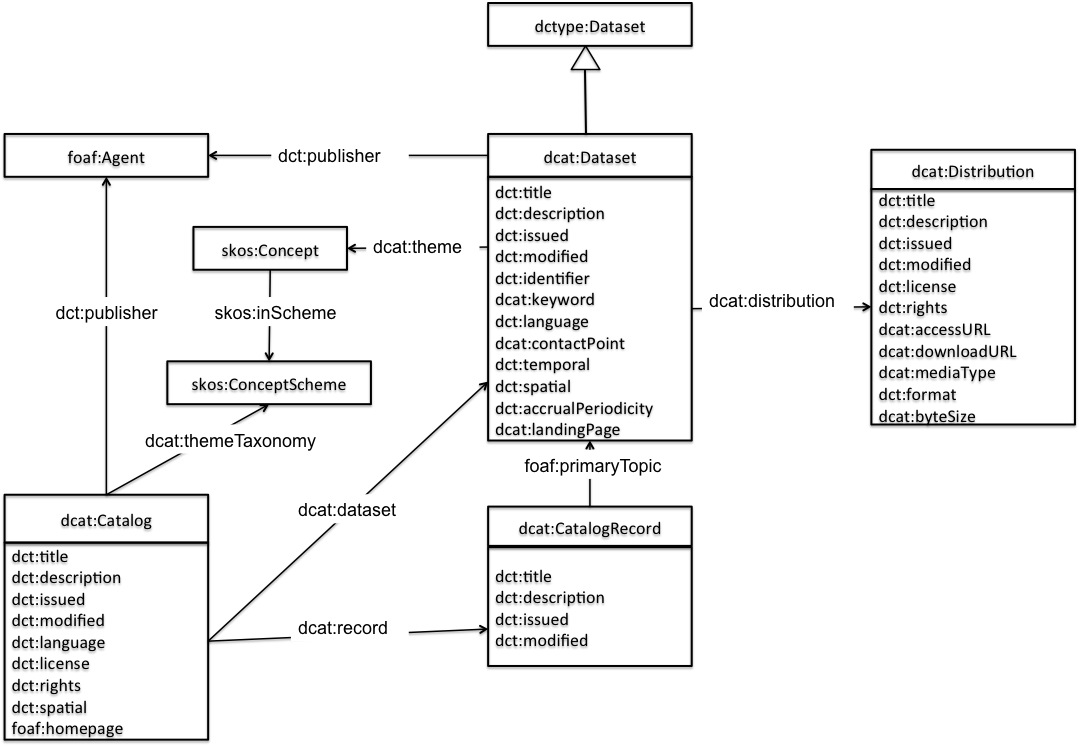
\includegraphics[scale=0.40]{img/dcatmodel.jpg}
\caption{Modello DCAT}
\end{center}
\end{figure}

\newpage
\subsection{DCAT-AP e DCAT-AP-it}
Il DCAT Application Profile (DCAT-AP) fornisce una specifica comune per la descrizione di dati della pubblica amministrazione in Europa, questa specifica è basata sullo standard DCAT: Data Catalog Vocabulary. \footnotemark
\footnotetext{https://www.w3.org/TR/vocab-dcat}
\\
\\
DCAT-AP-it è la versione italiana di DCAT-AP, il profilo nazionale dei metadati utili per descrivere i dati delle pubbliche amministrazioni, conforme alla specifica di DCAT-AP serve a favorire l'interoperabilità semantica di dati e servizi. DCAT-AP-it è un modello dati pensato per rendere omogenei in tutta la pubblica amministrazione italiana i processi di accesso e scambio delle informazioni tra le istituzioni stesse e tra le istituzioni e i cittadini e le imprese, in coerenza con il relativo framework europeo. 
\\
\\
L'utilizzo di un modello dati valorizza il patrimonio informativo pubblico nazionale in linea con la Direttiva relativa al riutilizzo dell'informazione del settore pubblico.
\\
\\
Le categorie definite nel profilo europeo dei metadati DCAT-AP (categorizzazione adottata dal portale europeo European Data Portal) - sono le seguenti:

\begin{enumerate}
\item \textbf{AGRI:} Agriculture, Fisheries, Forestry \& Foods
\item \textbf{ENER:} Energy
\item \textbf{REGI:} Regions \& Cities
\item \textbf{TRAN:} Transport
\item \textbf{ECON:} Economy \& Finance
\item \textbf{INTR:} International Issues
\item \textbf{GOVE:} Government \& Public Sector
\item \textbf{JUST:} Justice, Legal System \& Public Safety
\item \textbf{EDUC:} Education, Culture \& Sport
\item \textbf{ENVI:} Environment
\item \textbf{HEAL:} Health
\item \textbf{SOCI:} Population \& Society
\item \textbf{TECH:} Science \& Technology
\end{enumerate}


\begin{figure}[htbp]
\begin{center}
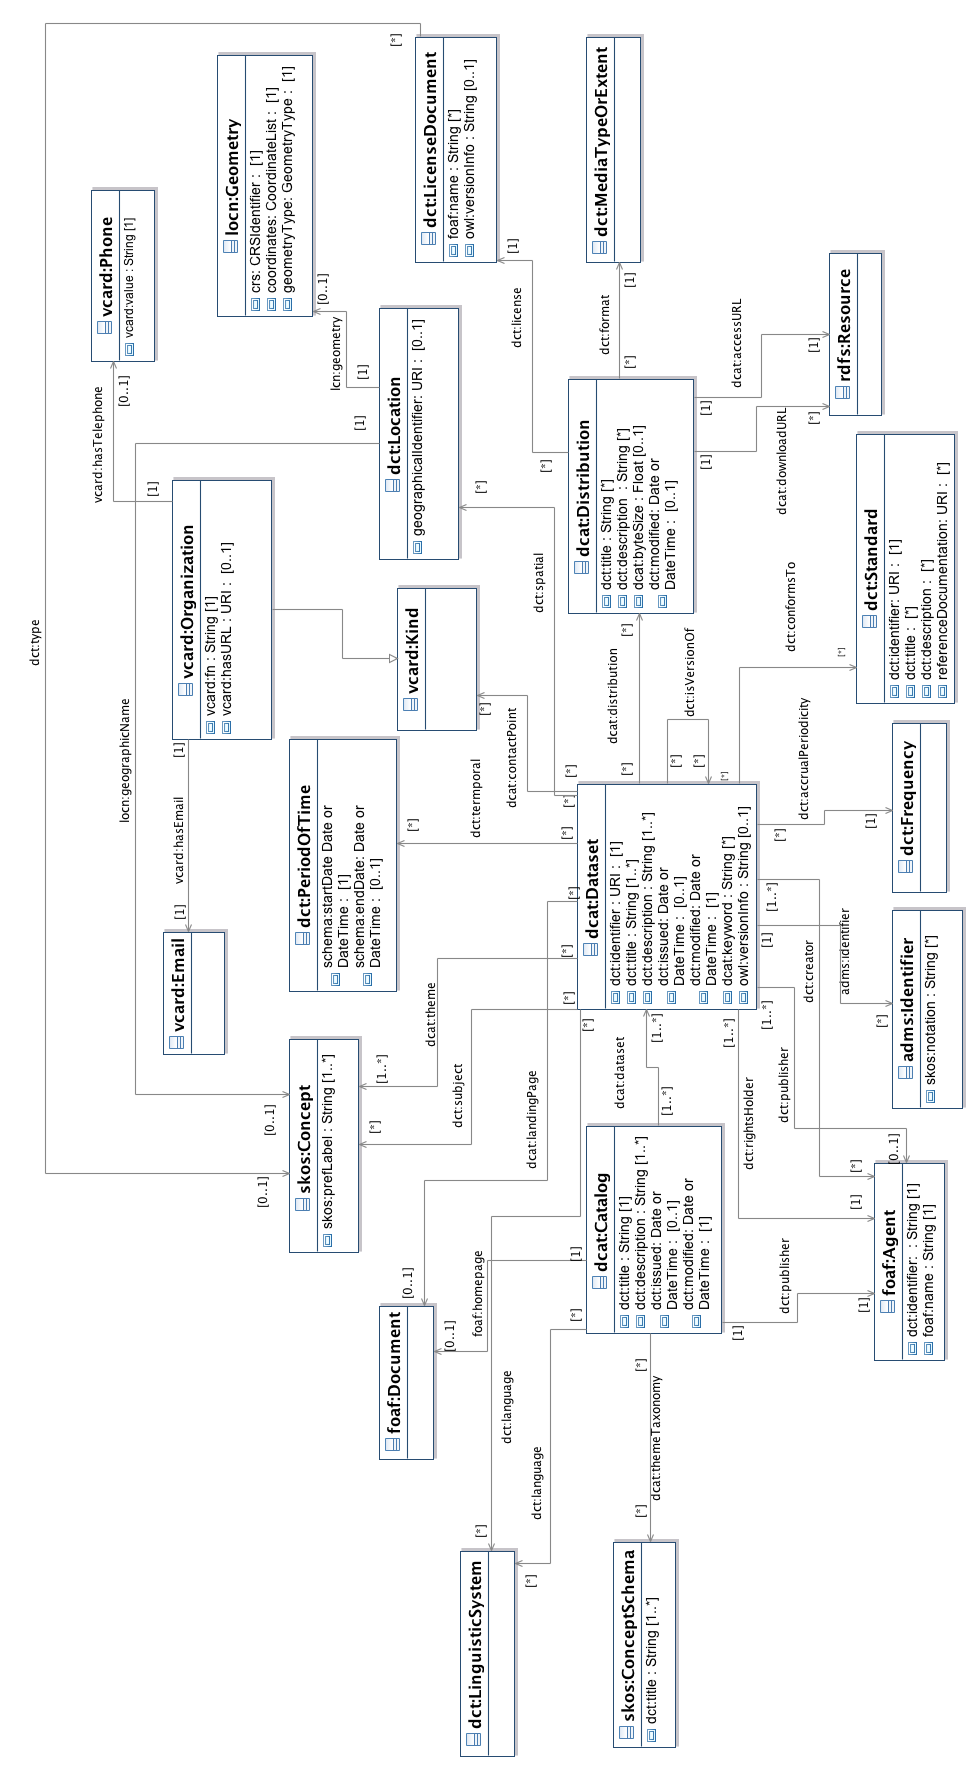
\includegraphics[scale=0.40]{img/DCAT-AP_IT_UML.png}
\caption{Modello dati DCAT-AP-it}
\end{center}
\end{figure}

\subsection{CKAN}
CKAN (Comprehensive Knowledge Archive Network) è un sistema open source (\url{https://github.com/ckan/ckan}) pensato per l'immagazzinamento, la catalogazione e la distribuzione dei dati in diversi formati; quali ad esempio fogli di calcolo, CSV, PDF, XML, RDF, ed altri tipi di file.
\\
\\
CKAN è scritto in Python ed è ispirato dal sistema di gestione dei pacchetti comune a sistemi operativi open source come quelli della famiglia Linux. CKAN è un sistema performante e manutenuto da una comunità di sviluppatori online (Open Knowledge Foundation).  
\\
\\
Il sistema è usato sia come piattaforma pubblica su Datahub (\url{https://datahub.io}), sia da varie pubbliche amministrazioni nell'ambito della loro strategia di pubblicazione di dati aperti, ogni portale web basato su CKAN espone delle API (Application programming interface) mediante le quali è possibile interrogare i dataset e fruire dei dati di ciascun portale. 
\\
\\
Molte pubbliche amministrazioni europee utilizzano CKAN (standard de facto) per la pubblicazione, gestione, e presentazione dei propri dati aperti. Riporto i link ad alcune pubbliche amministrazioni che utilizzano CKAN:
\begin{itemize}

\item \url{https://data.gov.uk}
\item \url{http://dati.emilia-romagna.it}
\item \url{http://dati.trentino.it}
\item \url{http://dati.comune.lecce.it}
\end{itemize}
Oltre alle amministrazioni esiste un portale europeo (anch'esso basato su CKAN):
\\
\\
\url{https://europeandataportal.eu}
\\
\\
Il portale europeo raccoglie i metadati delle informazioni del settore pubblico disponibili sui portali di dati pubblici dei vari paesi europei.
Come detto in precedenza il profilo DCAT-AP garantisce l'interoperabilità, CKAN salvaguarda questa importante caratteristica dei dati aperti mettendo a disposizione un'estensione (plugin):
\\
\\
\url{https://github.com/ckan/ckanext-dcat} 
\\
\\
Il plugin è pensato per abilitare l'esportazione dei metadati in formato DCAT. La corrispondenza tra i campi che descrivono i dati in CKAN ed i campi in DCAT è realizzata mediante un mapping:
\\
\\
\url{https://github.com/ckan/ckanext-dcat#rdf-dcat-to-ckan-dataset-mapping}
\\
\\
il quale prende i valori dai campi CKAN e li mappa in quelli DCAT.

\subsubsection{European Data Portal}
European Data Portal (\url{https://europeandataportal.eu}) è il portale europeo degli open-data dataset di tutta europa.
Il portale europeo oltre a raccogliere i metadati europei produce delle analisi riguardanti la fornitura di dati e i vantaggi del loro riutilizzo. In tutta Europa, i dati sono sempre più aperti e disponibile per il riutilizzo. 
\\
\\
Un certo numero di studi ha incrementato le aspettative per quanto riguarda i benefici finanziari dei dati aperti, la strada da percorrere per sfruttare pienamente i dati aperti è ancora lunga. Il portale europeo esplora approfonditamente il tema del riutilizzo dei dati aperti, al fine di sostenere la trasformazione dei dati in valore (economico, sociale e politico). 

\begin{figure}[htbp]
\begin{center}
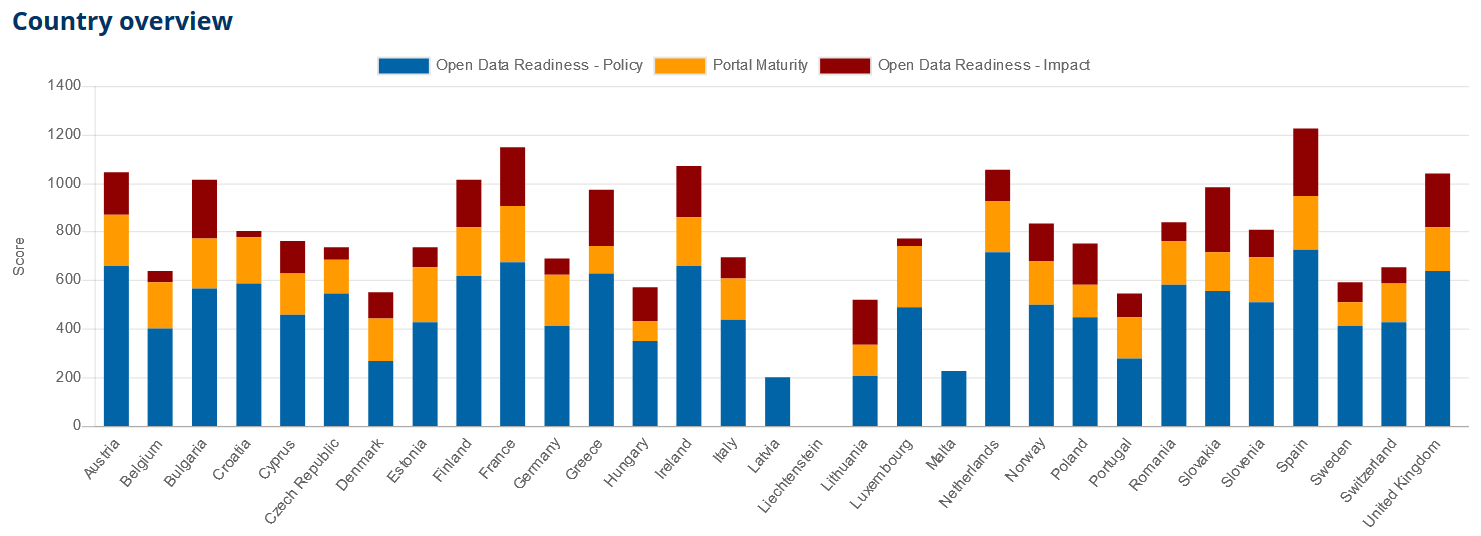
\includegraphics[scale=0.50]{img/eustat.png}
\caption{Alcune analisi prodotte dal portale europeo}
\end{center}
\end{figure}

\subsubsection{Open Data Hub Italy}
Open Data Hub Italy (\url{http://sciamlab.com/opendatahub/it}) è una piattaforma per l'indicizzazione e la ricerca di dati aperti (open-data), è il più grande portale italiano di raccordo dei dati aperti delle pubbliche amministrazioni italiane. 
\\
\\
Questo portale - anch'esso basato su CKAN - raccoglie più di 34'000 dataset, l'ammontare dei dati e delle organizzazioni tracciate cresce continuamente in quanto il ciclo di aggiornamento del catalogo è contenuto grazie all'utilizzo di algoritmi di processamento parallelo e distribuito.
\\
\\
La piattaforma utilizza algoritmi basati su esecuzione parallela per l'analisi dei testi, l'arricchimento dei metadati di categoria - è realizzato automaticamente mediante il classificatore JRC-JEX (categorizzazione con le voci del tesauro EuroVoc).
\\
\\
Nella fase di harvesting, quando i dati non sono disponibili in maniera esplicita (mediante API), si utilizzano tecniche di \say{scraping} per reperire le informazioni direttamente dal codice HTML.
\subsubsection{Dati.gov.it}
Il portale Dati.gov.it (\url{http://dati.gov.it}) è il portale ufficiale dei dati aperti italiani, raccoglie circa 10'000 dataset open-data, è il portale italiano che fornisce i dati italiani al portale europeo. Il portale italiano è gestito dall'Agenzia per l'Italia digitale, la quale fornisce anche le linee guida per la modellazione del profilo italiano dei metadati DCAT-AP-it.

\subsection{EuroVoc}
EuroVoc è un tesauro multilingue e pluridisciplinare che comprende la terminologia dei settori d'attività dell'Unione europea. Contiene termini in 23 lingue dell'UE. EuroVoc è in linea con le raccomandazioni del W3C e con gli ultimi sviluppi negli standard di classificazione. 
\\
\\
Il thesaurus EuroVoc viene utilizzato dalle istituzioni dell'Unione europea, dall'Ufficio delle pubblicazioni dell'UE, da parlamenti nazionali e regionali in Europa, come pure da amministrazioni nazionali e utenti privati di tutto il mondo.
\footnotemark
\footnotetext{http://eurovoc.europa.eu}
\\
\\
I descrittori del thesaurus multilingua EuroVoc sono usati da molti parlamentari europei e centri di documentazione per indicizzare manualmente le loro collezioni di documenti, i descrittori assegnati ai documenti sono utilizzati per cercare ed individuare documenti in una gerarchia semantica divisa in 21 domini, 127 sottodomini (microtesauri) e circa 7000 descrittori (concetti).
\\
\\
I 127 microtesauri di EuroVoc sono riconducibili alle 13 categorie DCAT-AP attraverso un mapping (più dettagli al paragrafo 2.7.4)
\newpage
\subsection{JRC-Acquis 3.0}
JRC-Acquis è un corpus parallelo multilingua che contiene documenti di natura governativa (riguardanti varie tematiche) utilizzati/prodotti dalle istituzioni europee.  
La versione corrente di JRC-Acquis (3.0) contiene più di 23'000 documenti annotati manualmente con i descrittori dei concetti del tesauro EuroVoc. 
\\
\\
\url{https://ec.europa.eu/jrc/en/language-technologies/jrc-acquis}
\\
\\
JRC-Acquis può essere usato per addestrare e/o testare sistemi di classificazione basati su algoritmi di text mining o software per la keyword-assignment basati su varie tecnologie semantiche. Il corpus è codificato in XML, in accordo con lo standard TEI per la descrizione dei campi.
\footnotemark
\footnotetext{Steinberger, Ebrahim, Poulis, Carrasco-Benitez, Schlüter, Przybyszewski \& Gilbro. An overview of the European Union's highly multilingual parallel corpora. Language Resources and Evaluation Journal, JRC, 2014}
\begin{figure}[htbp]
\begin{center}
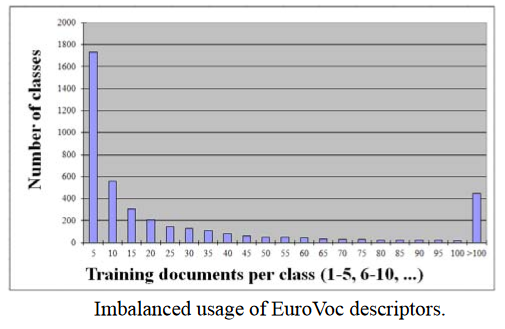
\includegraphics[scale=1.00]{img/evocimbalanced.png}
\caption{Utilizzo dei descrittori EuroVoc in JRC-Acquis}
\end{center}
\end{figure}
\phantom
\\
Alcuni descrittori sono utilizzati molto di più rispetto ad altri all'interno del corpus Acquis, 1733 descrittori sono utilizzati 5 volte o meno di 5 volte nei documenti, 355 descrittori sono utilizzati tra le 50 e le 100 volte, 420 descrittori sono utilizzati tra il centinaio e il migliaio di documenti. Questo sbilanciamento nell'utilizzo dei descrittori rappresenta una grande sfida nel contesto della classificazione basata sui descrittori del tesauro EuroVoc (vedi classificatore JRC-JEX)
\begin{figure}[htbp]
\begin{center}
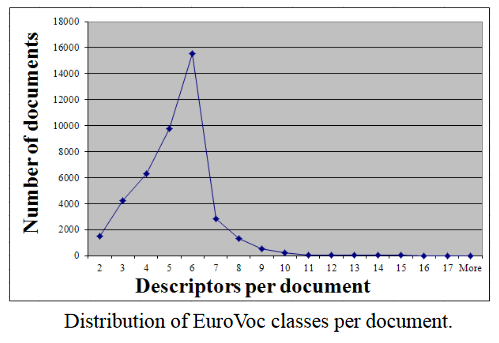
\includegraphics[scale=1.00]{img/evocdistribution.png}
\caption{Utilizzo dei descrittori EuroVoc per documento in JRC-Acquis}
\end{center}
\end{figure}
Ciascun documento di Acquis è etichettato con 5.43 (in media) descrittori EuroVoc, con una deviazione standard di 1.86.
\footnotemark
\footnotetext{Steinberger, Ebrahim, Turchi. JRC EuroVoc Indexer JEX - A freely available multi-label categorisation tool. European Commission, JRC, 2014}
\\
\\
Come anticipato nel paragrafo 2.6 e dettagliato nel paragrafo 2.7.4 i descrittori di EuroVoc sono riconducibili alle 12 categorie Eu-Data-Themes (DCAT-AP), così facendo il corpus JRC-Acquis può essere utilizzato per il task di classificazione su DCAT-AP (12 categorie), il corpus che si ottiene è sempre multi-label (ogni documento ha 3.47 categorie DCAT-AP).
\\
\\
Riporto di seguito il numero di volte che occorrono le varie categorie Eu-Data-Themes (DCAT-AP) tra i circa 23'000 documenti etichettati con i descrittori EuroVoc:

\begin{figure}[htbp]
\begin{center}
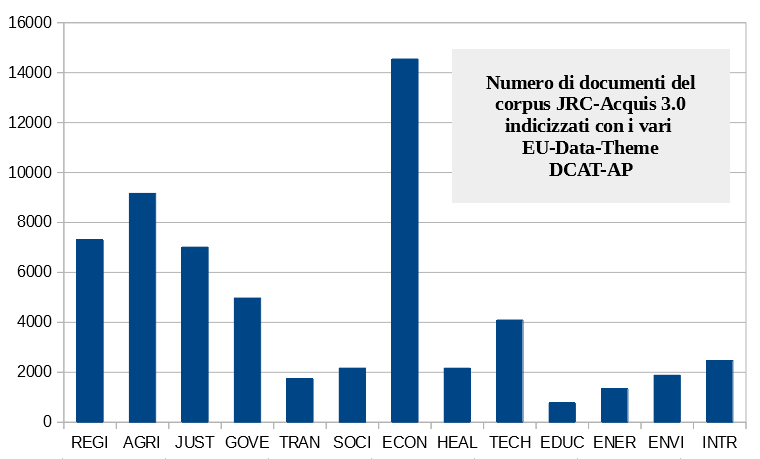
\includegraphics[scale=0.70]{img/numacquis.png}
\caption{Documenti di Acquis 3.0 indicizzati con EU-Data-Themes}
\end{center}
\end{figure}
\begin{verbatim}
REGI, 7314; AGRI, 9164; JUST, 7012; GOVE, 4973; TRAN, 1739;
SOCI, 2167; ECON, 14544; HEAL, 2165; TECH, 4093; EDUC, 775;
ENER, 1350; ENVI, 1882; INTR, 2474
\end{verbatim}
\phantom
\\
I vantaggi che possiamo trarre utilizzando JRC-Acquis come corpus di addestramento per la catalogazione di open-data con le categorie DCAT-AP sono molteplici, tra i vantaggi principali abbiamo: 

\begin{enumerate}
\item Standard TEI
\item Corpus aggiornato e manutenuto
\item Corpus multilingua
\item Bridge dinamico tra i concetti e le categorie DCAT-AP
\end{enumerate}

\subsubsection{Standard TEI}
JRC-Acquis ha un formato che rispetta lo standard TEI.
Text Encoding Initiative (TEI) è un consorzio che sviluppa e mantiene uno standard per la rappresentazione di testi in formato digitale. La codifica TEI garantisce che il corpus sia machine-readable,  le modalità di interazione dei sistemi che utilizzano JRC-Acquis (ad esempio un modulo XQuery) non variano al variare delle versioni di JRC-Acquis.
\\
\\
Il titolo del documento è contenuto nel tag head:
\begin{verbatim}
<head n="1"> 
   Decisione n. 2046/2002/CE del Parlamento europeo e del Consiglio,
   del 21 ottobre 2002, che modifica la decisione n. 1719/1999/CE
   relativa ad una serie di orientamenti, compresa l'individuazione 
   di progetti di interesse comune, per reti transeuropee per lo 
   scambio elettronico di dati fra amministrazioni (IDA)
</head>
\end{verbatim}
Il corpo testuale del documento è contenuto nel tag div di tipo body
\begin{verbatim}
<div type="body">
   ...
</div>
\end{verbatim}
Segue la parte relativa alla classificazione EUROVOC:
\begin{verbatim}
<profileDesc>
   <textClass>
      <classCode scheme="eurovoc">206</classCode>
      <classCode scheme="eurovoc">3010</classCode>
      <classCode scheme="eurovoc">453</classCode>
      <classCode scheme="eurovoc">616</classCode>
      <classCode scheme="eurovoc">4424</classCode>
      <classCode scheme="eurovoc">5864</classCode>
   </textClass>
</profileDesc>
\end{verbatim}
Ogni documento contiene anche dei metadati come la data di emissione dei documenti:
\begin{verbatim}
<date>
   2007-03-29
</date>
\end{verbatim}
e la sorgente:
\begin{verbatim}
<div type="signature">
   <p n="77">Fatto a Lussemburgo, addì 21 ottobre 2002.</p>
   <p n="78">Per il Parlamento europeo</p>
   <p n="79">Il Presidente</p>
   <p n="80">P. Cox</p>
   <p n="81">Per il Consiglio</p>
   <p n="82">Il Presidente</p>
   <p n="83">P. S. Møller</p>
   <p n="84">(1) GU C 332 E del 27.11.2001, pag. 287.</p>
   <p n="85">(2) GU C 80 del 3.4.2002, pag. 21.</p>
   ... 
</div>
\end{verbatim}

\subsubsection{Corpus aggiornato e manutenuto}
JRC-Acquis è un corpus manutenuto e aggiornato manualmente, decine di migliaia di documenti riguardanti politiche europee su tematiche trasversali sono arricchiti da descrittori EuroVoc da specialisti del dominio. JRC-Acquis viene manutenuto perché utilizzato da diversi sistemi basati su tecnologie semantiche, nell'ambito della classificazione è utilizzato come corpo di addestramento del classificatore JRC-JEX, sistema ufficiale di classificazione dei documenti utilizzato dal parlamento europeo.

\subsubsection{Corpus parallelo multilingua}
JRC-Acquis è un corpus multilingua, questo vuol dire che è disponibile una versione per ciascuna lingua dell'Unione Europea. Il parallelismo è dato dal fatto che molti documenti sono disponibili in più lingue. Utilizzare corpus multilingua facilita il compito di sviluppare sistemi basati su tecnologie semantiche multilingua.

\newpage
\subsubsection{Bridge dinamico tra EuroVoc e le categorie DCAT-AP}
\begin{figure}[htbp]
\begin{center}
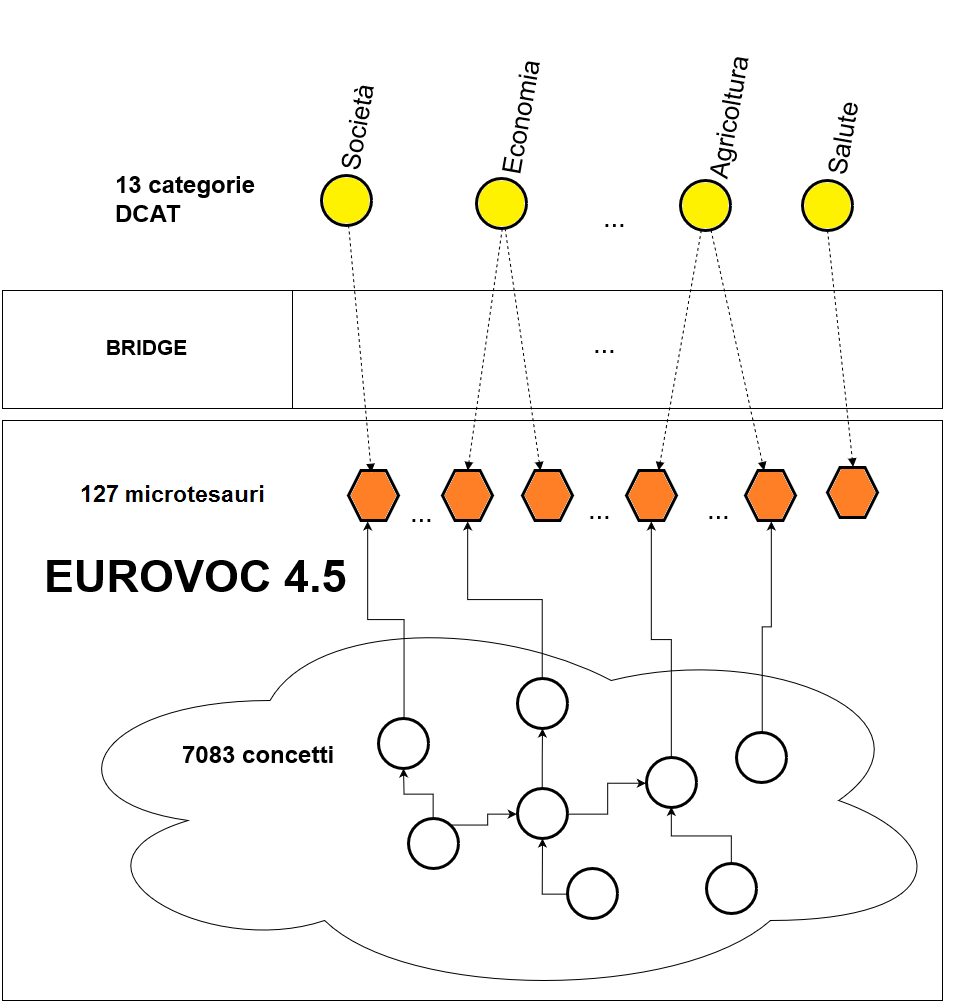
\includegraphics[scale=0.30]{img/eurovocdcat.png}
\caption{Bridge tra le categorie DCAT-AP ed EUROVOC}
\end{center}
\end{figure}

In appendice (\say{Associazione dei Temi DCAT-Microtesauri EuroVoc}) è possibile prendere nota delle corrispondenze tra i 13 temi definiti nell'ambito di DCAT-AP e i concetti (microtesauri) disponibili nel vocabolario EuroVoc (come indicato dal portale europeo https://www.europeandataportal.eu).
\footnotetext{Profilo italiano di DCAT-AP (DCAT Application Profile for data portals in Europe), Versione 1.0, Agenzia per l'Italia digitale, 2006}
\\
\\
JRC-Acquis è indicizzato con i concetti del vocabolario EuroVoc, pertanto è stato necessario sviluppare un modulo specializzato per la navigazione del tesauro al fine di ottenere i descrittori dei microtsauri associati ai descrittori dei concetti, per poi permutarli a loro volta nei rispettivi temi DCAT-AP.
\\
Il seguente modulo java:
\url{https://github.com/simonegasperoni/cata/blob/master/code/src/main/java/com/sciamlab/it/eurovoc/EVoc.java}
\\
è dedicato alla gestione di EuroVoc, fornisce funzionalità di base per interrogare il tesauro:
\begin{enumerate}
\item Dato un concetto si ottengono i microtesauri associati
\item Dato un microtesauro si ottiene il relativo tema DCAT-AP (EU Data Theme) 
\end{enumerate}

Un corpus etichettato con le voci di un tesauro come EuroVoc permette la realizzazione di associazioni tra concetti a vario livello di astrazione in modo dinamico, ad esempio qualora il microtesauro EuroVoc \say{2831 culture and religion} originariamente associato al tema Population \& Society (Popolazione e Società) dovesse passare in Education, culture and sport (Educazione, cultura e sport), basterebbe modificare il mapping tra i microtesauri e i temi all'interno del modulo specializzato.
\begin{lstlisting}
Map<String, EUNamedAuthorityDataTheme.Theme> EUROVOC_TO_DCAT_CATEGORIES = new HashMap<String, EUNamedAuthorityDataTheme.Theme>(){
		{
			put("0406",EUNamedAuthorityDataTheme.Theme.GOVE); 		
			...
			...
			...
			put("7626",EUNamedAuthorityDataTheme.Theme.INTR); 	
		}
};
\end{lstlisting}

Il tesauro (EuroVoc) e il corpus (JRC-Acquis) sono i due componenti fondamentali per la costruzione dei dati di addestramento del classificatore, essendo questi due componenti disaccoppiati è possibile pensare di aggiornare uno e mantenere immutato l'altro qualora siano disponibili versioni più aggiornate del corpus o del tesauro. Anche questa è una forma di flessibilità, anche se in realtà dall'aggiornamento del tesauro non si traggono benefici se i descrittori dei concetti aggiunti non compaiono anche nel corpus. 
\newpage
\subsection{JRC-JEX: il classificatore EuroVoc}
Il classificatore JEX, sviluppato presso i laboratori JRC (Joint Research Centre) è stato presentato nell'ambito del workshop \say{Ontologies and Information Extraction at EUROLAN 2003: The Semantic Web and Language Technology – Its Potential and Practicalities}. 
\\
\\
JEX è un classificatore multi-label, addestrato con il corpus JRC-Acquis (training set), categorizza con i descrittori (concetti) del tesauro EuroVoc con tecniche basate sull'approccio \say{VSM} (vector space model).
La scelta di basare il classificatore su EuroVoc e JRC-Acquis rende il sistema multilingua e garantisce la copertura di tutte le tematiche di interesse della politica europea.
\\
\\
Riporto di seguito le performance registrate sulle lingue coperte dal classificatore, le metriche sono descritte in dettaglio nel capitolo 6.
\begin{figure}[htbp]
\begin{center}
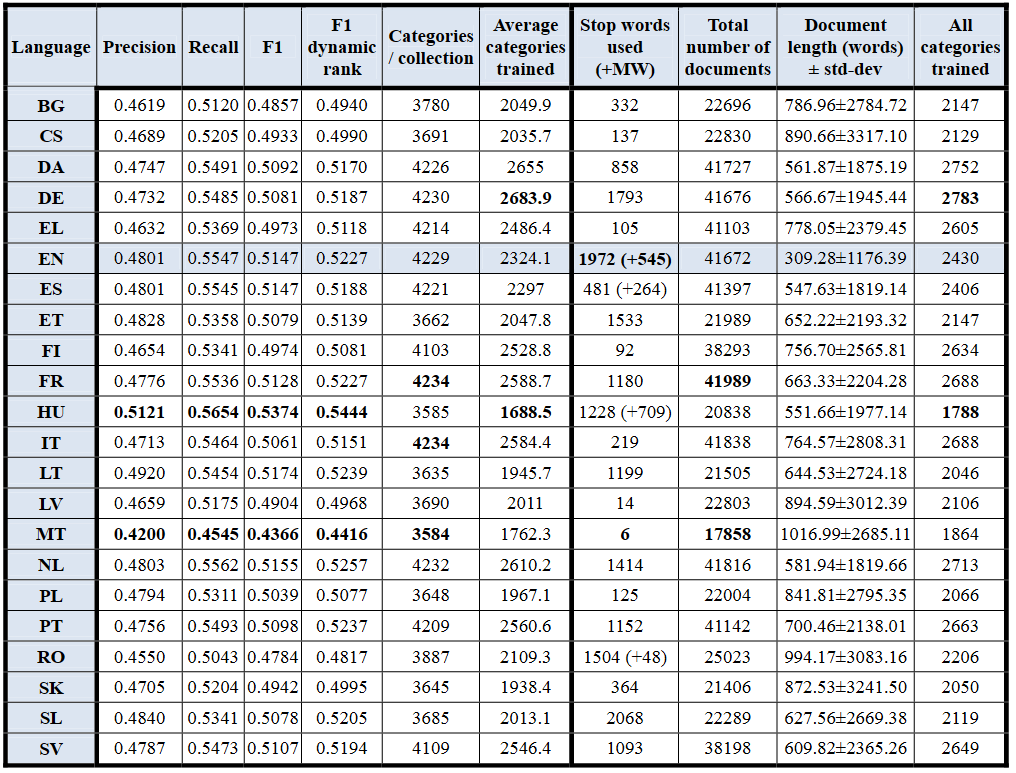
\includegraphics[scale=0.70]{img/statjex.png}
\caption{Evaluation multilingua di JEX}
\end{center}
\end{figure}
\newpage
\section{Elaborazione del corpus}
Una fase preliminare in qualsiasi ambito di classificazione di documenti è l'elaborazione dei corpi testuali, si tratta di scegliere le modalità con le quali estrarre le \say{feature} dai testi - in base alla loro formattazione, al fine di rendere le \say{feature} fruibili al sistema di classificazione in modo opportuno.
\\
\\
Nel contesto di un sistema di categorizzazione dei testi vogliamo ottenere delle \say{feature} ben rappresentative del contenuto semantico dei documenti dai quali sono estratte. Le tappe che dobbiamo percorrere sono essenzialmente due: innanzitutto è necessario utilizzare degli algoritmi per l'estrazione di \say{feature}, dopodiché queste \say{feature} potranno essere stemmerizzate o rielaborate in vario modo, ad esempio utilizzando n-grammi di parole. 
\\
\\
Il processo di elaborazione viene suddiviso in fasi diverse, tuttavia simili a quelle che si possono incontrare nel processo di elaborazione di un linguaggio di programmazione, i seguenti passi rappresentano un possibile canovaccio da seguire per l'elaborazione dei testi:

\begin{itemize}
\item \textbf{Analisi lessicale:} scomposizione di un'espressione linguistica in token (in questo caso le parole).
\item \textbf{Analisi grammaticale:} associazione delle parti del discorso a ciascuna parola nel testo.
\item \textbf{Analisi sintattica:} arrangiamento dei token in una struttura sintattica (ad albero: parse tree).
\item  \textbf{Analisi semantica:} assegnazione di un significato (semantica) alla struttura sintattica e, di conseguenza, all'espressione linguistica.
\end{itemize}


\subsection{Lemmatizzazione}
Una tecnica di elaborazione delle \say{feature} è la lemmatizzazione, vale a dire, \say{quel complesso di operazioni che conducono a riunire tutte le forme sotto il rispettivo lemma}, intendendo per lemma \say{ciascuna parola-titolo o parola-chiave di un dizionario} e per forma ogni possibile diversa realizzazione grafica di un lemma.\footnotemark
\footnotetext{Busa, Fondamenti di informatica linguistica, Istituto Geografico De Agostini, 1987}
\\
\\
Esistono delle convenzioni di lemmatizzazione proprie di ciascuna lingua: ad esempio in italiano è uso convenzionale che il lemma verbale sia la forma coniugata all'infinito presente attivo.
\\
La lemmatizzazione è, dunque, una pratica apparentemente facile, se non, addirittura, ovvia ed intuitiva: più, o meno tutti, infatti, esercitiamo quotidianamente la conoscenza della differenza tra lemma e forma. Tuttavia, alla prova dei fatti, la lemmatizzazione rivela una serie di problemi, il più delle volte non immaginabili prima di averne fatto esperienza diretta: queste difficoltà rendono il lemmatizzare un esercizio interessante, in quanto costringe chi lo esercita a riflettere su:

\begin{itemize}  
\item Quanti e quali automatismi l'uomo metta inconsciamente in atto ogni volta che parla, o scrive.
\item Quanto sia difficile formalizzare questi automatismi.
\end{itemize}

Esistono due tipi di lemmatizzazione: la lemmatizzazione morfologica analizza le forme di parole in isolamento, ovvero fuori dal contesto sintattico, fornendone tutti i valori che sono possibili in un dato sistema linguistico. 
\\
\\
La lemmatizzazione morfo-sintattica analizza le forme di parole entro il contesto sintattico. Non è mai ambigua, ma sempre univoca, in quanto l'immersione della forma nella frase ne precisa il valore. Quindi, mentre la lemmatizzazione morfologica è indipendente dal testo, la lemmatizzazione sintattica è, invece, legata al contesto.
\\
\\
Questo processo è reso particolarmente difficile e complesso a causa delle caratteristiche intrinseche di ambiguità del linguaggio umano. Il problema della lemmatizzazione richiama il problema della disambiguazione, infatti talvolta nell'assegnazione dei lemmi ai termini è necessario contestualizzare il termine.



\subsection{Disambiguazione}
Nell'analisi semantica la procedura automatica che attribuisce all'espressione linguistica un significato tra i diversi possibili è detta disambiguazione.
La comprensione del linguaggio naturale è spesso considerata un problema IA-completo, poiché si pensa che il riconoscimento del linguaggio richieda una conoscenza estesa del mondo e una grande capacità di manipolarlo. Per questa ragione, la definizione di \say{comprensione} è uno dei maggiori problemi dell'elaborazione del linguaggio naturale.\footnotemark
\footnotetext{Chiari, Introduzione alla linguistica computazionale, Laterza, 2007}
\\
\\
Molte parole nel linguaggio naturale sono delle polisemie, vale a dire, possono avere più significati. Le tecniche finalizzate alla disambiguazione sono conosciute in letteratura come \textit{Word Sense Disambiguation} (WSD).
\\
\\
La WSD può essere affrontata come un problema di classificazione, il senso corretto è la classe da predire la parola è rappresentata con un insieme (vettore) di feature in ingresso al classificatore, l'ingresso è di solito costituito da una rappresentazione della parola da disambiguare (target) e del contesto in cui si trova (un certo numero di parole a sinistra e destra della parola target). Il classificatore può essere stimato con tecniche di apprendimento automatico a partire da un dataset etichettato. Si possono usare diversi modelli per costruire il classificatore (Naïve Bayes, reti neurali, alberi di decisione...).
\\
\\
Il problema dell'approccio appena descritto è che il modello di apprendimento supervisionato che scegliamo di adottare potrebbe richiedere un training set troppo grande per essere sufficientemente preciso, per questo motivo esistono tecniche alternative come i metodi Dictionary-based.
\\
\\
Tra i metodi Dictionary-based abbiamo l'algoritmo di Lesk (1986) che è un metodo molto semplice, basato sull'intuizione secondo cui un dizionario può fornire informazioni sul contesto legato ai sensi delle parole (le glosse).  

 
\subsection{Stemming}
Lo stemming è il processo usato per ridurre parole flesse al loro tema, il tema non deve necessariamente coincidere con la radice morfologica della parola: l'importante è che parole con una semantica strettamente correlata vengano mappate sullo stesso tema. Le tecniche di stemming sono studiate in informatica da quarant'anni, sono uno dei metodi di base per ridurre la dimensionalità dei documenti di testo.
\\
\\
In questo campo è stato fondamentale il contributo di Martin Porter, inventore dello \say{stemmer di Porter}, uno dei più comuni algoritmi per la stemmerizzazione in lingua inglese, e inventore del framework Snowball:
\\
\url{http://snowballstem.org}
\\
\\
Porter definì il suo algoritmo di stemming in un articolo del 1980 \say{An algorithm for suffix stripping}, il quale è stato citato più di 8'000 volte secondo Google Scholar.

\subsection{Snowball}
\textit{
Since it effectively provides a \say{suffix STRIPPER GRAMmar}, I had toyed with the idea of calling it \say{strippergram}, but good sense has prevailed, and so it is \say{Snowball} named as a tribute to SNOBOL, the excellent string handling language of Messrs Farber, Griswold, Poage and Polonsky from the 1960s.
\\
Martin Porter
}
\\
\\
Il progetto Snowball è un progetto open source:
\\
\url{https://github.com/snowballstem/snowball}
\\
Il progetto Snowball raccoglie le implementazioni di vari algoritmi di stemming (per più lingue e in più linguaggi di programmazione). Snowball è utilizzato in diversi progetti Apache Software Foundation, tra i quali abbiamo Apache Solr e Apache Lucene.
\\
Le stopword della lingua italiana sono riportate in formato txt al seguente indirizzo:
\\
\url{http://snowballstem.org/algorithms/italian/stop.txt}
\\
\\
Tartarus Snowball contiene anche un adattamento dell'algoritmo di Porter per la lingua italiana, riporto di seguito l'algoritmo di stemming per la lingua italiana:
\\
\\
La lingua italiana prevede le seguenti forme accentate:
\\
\\
\textit{á, é, í, ó, ú, à, è, ì, ò, ù}
\\
\\
Gli accenti acuti vanno rimpiazzati con gli accenti gravi. Le vocali sono:
\\
\\
\textit{a, e, i, o, u, à, è, ì, ò, ù}
\\
\\
Nell'algoritmo di stemming della lingua italiana - ma non solo - si utilizzano le due seguenti definizioni di \say{regione}: 

\begin{itemize}
\item \textbf{R1}: è la regione che segue la prima non vocale seguita da una vocale, potrebbe essere nulla qualora non ci fosse una non vocale.
\item \textbf{R2}: è la regione che segue la prima non vocale seguita da una vocale nella regione R1, anche questa potrebbe essere una regione nulla.
\item \textbf{RV}: Se la seconda lettera è una consonante, RV è la regione che segue la prossima vocale, oppure se le prime due lettere sono vocali, RV è la regione che segue la prossima consonante; altrimenti (nel caso consonante-vocale) RV è la regione dopo la terza lettera.
\end{itemize}
Riporto di seguito i passi dell'algoritmo:
\begin{enumerate}
\item Ricerca del più lungo suffisso tra i seguenti:
\\
\textit{ci, gli, la, le, li, lo, mi, ne, si, ti, vi, sene, gliela, gliele, glieli, glielo, gliene, mela, mele, meli, melo, mene, tela, tele, teli, telo, tene, cela, cele, celi, celo, cene, vela, vele, veli, velo, vene}
\\
\\
a seguito di questi altri suffissi:
\\
\\
(a) \textit{ando, endo}
\\
(b) \textit{ar, er, ir}
\\
\\
In RV, nel caso di (a) il suffisso è cancellato, nel caso di (b) è rimpiazzato dalla \say{e}:
\\
\\
Ad esempio abbiamo:
\\
guardandogli → guardando
\\
accomodarci → accomodare
\\
\item Ricerca del più lungo suffisso tra i seguenti suffissi:
\\
Cancellare se in R2:
\\
\textit{anza, anze, ico, ici, ica, ice, iche, ichi, ismo, ismi, abile, abili, ibile, ibili, ista, iste, isti, istà,  istè, istì, oso, osi, osa, ose, mente, atrice, atrici, ante, anti}
\\
\\
Cancellare se in R2:
\\
\textit{azione, azioni, atore, atori} 
\\
\\
Sostituire con \textit{log}, se in R2:
\\ 
\textit{logia, logie}
\\
\\
Sostituire con \textit{u}, se in R2:
\\
\textit{uzione, uzioni, usione, usioni} 
\\
\\
Sostituire con \textit{ente}, se in R2:
\\
\textit{enza, enze}  
\\
\\
Cancellare se in RV:
\\
\textit{amento, amenti, imento, imenti}
\\
\\
Cancellare \textit{amente} se in R1
\\
se preceduto da \textit{iv}, cancellare se in R2 (anche se preceduto da \textit{at}, cancellato se in R2), altrimenti, se preceduto da \textit{os, ic, abil} cancellare se in R2 
\\
\\
Cancellare \textit{ità} se preceduto da \textit{abil, ic, iv} in R2
\\
\\
Cancellare \textit{ivo, ivi, iva, ive} in R2 
\\
\\
Si passa al passo tre se non abbiamo più nulla da rimuovere.

\item Per quanto riguarda i suffissi dei verbi si va alla ricerca del più lungo suffisso in RV, e, se trovato, si cancella:
\\
\\
\textit{ammo, ando, ano, are, arono, asse, assero, assi, assimo, ata, ate, ati, ato, ava, avamo, avano, avate, avi, avo, emmo, enda, ende, endi, endo, erà, erai, eranno, ere, erebbe, erebbero, erei, eremmo, eremo, ereste, eresti, erete, erò, erono, essero, ete, eva, evamo, evano, evate, evi, evo, Yamo, iamo, immo, irà, irai, iranno, ire, irebbe, irebbero, irei, iremmo, iremo, ireste, iresti, irete, irò, irono, isca, iscano, isce, isci, isco, iscono, issero, ita, ite, iti, ito, iva, ivamo, ivano, ivate, ivi, ivo, ono, uta, ute, uti, uto, ar, ir}
\\
\\
\item Cancellare \textit{a, e, i, o, à, è, ì} oppure \textit{ò} se in RV
\\
\\
crocchi → crocch
\\
crocchio → crocch 
\\
\\
Sostituire infine \textit{ch, gh} con \textit{c, g} se in RV 
\\
\\
crocch → crocc 

\end{enumerate}

\begin{verbatim}
public List<String> execute(String text){
    String resultString = text.replaceAll("\\P{L}+", " ").toLowerCase();
    List<String> result=new ArrayList<String>();
    StringTokenizer tk=new StringTokenizer(resultString);
    while(tk.hasMoreTokens()){
        String s=tk.nextToken(); 
        if(!stopwords.contains(s)){
            result.add(this.stems(s));
        }
    }
    return result;
}
\end{verbatim}


\newpage
\section{Algoritmi di classificazione}
\subsection{Tassonomia degli algoritmi di classificazione}

\subsection{Classificatori bayesiani naïve}
I classificatori bayesani sono metodi statistici di classificazione, predicono la probabilità che una data istanza appartenga ad una certa classe.
\\
\\
Nel gergo della classificazione di testi (o Text Categorization), con il termine classificatore bayesiano ci si riferisce convenzionalmente al classificatore bayesiano naïve (Naïve Bayes Classifier), ossia un classificatore bayesiano semplificato con un modello di probabilità sottostante che si basa sull'ipotesi di indipendenza delle feature, ovvero assume che la presenza o l'assenza di una particolare feature in un documento testuale non sia correlata alla presenza o assenza di altre feature.
\\
\\
I classificatori bayesiani sono metodi incrementali: ogni istanza dell'insieme di addestramento modifica in maniera incrementale la probabilità che una ipotesi sia corretta.
La conoscenza già acquisita può essere combinata facilmente con le nuove osservazioni basta aggiornare i conteggi. Questi metodi sono utilizzati ad esmpio in Mozilla o SpamAssassin per riconoscere le mail spam dalle mail ham.
\subsection{Assunzioni di indipendenza delle feature}
L'assunzione di indipendenza rende i calcoli possibili, consente di ottenere classificatori ottimali quando è soddisfatta. La condizione di indipendenza delle feature è, purtroppo, raramente soddisfatta in pratica, tuttavia, si è visto che anche quando l'ipotesi di indipendenza non è soddisfatta, i classificatori Naïve Bayes spesso forniscono ottimi risultati.
\\
\\
La probabilità dell'intersezione di due eventi indipendenti $E1$ ed $E2$ è data dal prodotto delle probabilità di ciascun evento, ovvero:
$$ P(E1 \cap E2) = P(E1) \cdot P(E2)$$
Se invece siamo di fronte a due eventi dipendenti, sappiamo che il verificarsi dell'uno, ad esempio di $E1$, influisce sul calcolo del verificarsi dell'altro, ad esempio $E2$. Si parlerà in tal caso di probabilità condizionata, $P(E2|E1)$.
\\
La probabilità dell'intersezione di due eventi dipendenti $E1$ e di $E2$ è data dal prodotto della probabilità di un evento per la probabilità condizionata dell'altro, cioè: 
$$ P(E1 \cap E2) = P(E1) \cdot P(E2|E1)$$
$E1$ e $E2$ possono essere invertiti, cioè:
$$ P(E1 \cap E2) = P(E2) \cdot P(E1|E2)$$

\begin{defn}
	La probabilità condizionale è definita come: $$P(B|A)=\frac{P(B \cap A)}{P(A)}$$
\end{defn}
\begin{defn}
	A e B sono condizionalmente indipendenti se $$P(B|A)=P(B)$$ o il suo equivalente $$P(A|B)=P(A)$$
\end{defn}
\subsection{Formula di Bayes}
Il teorema di Bayes (formula di Bayes o teorema della probabilità delle cause), proposto da Thomas Bayes, deriva da due teoremi fondamentali delle probabilità: il teorema della probabilità composta e il teorema della probabilità assoluta. Viene impiegato per calcolare la probabilità di una causa che ha scatenato l'evento verificato.
\\
\\
\textbf{Teorema di Bayes}
\\
\textit{
Dati gli eventi $A_j$ $\forall j$, stocasticamente indipendenti, vale a dire:
$$E \subset \bigcup\limits_{j=1}^{n} A_j $$
si dice che gli eventi $A_j$ sono la causa di $E$,  abbiamo dunque:
$$
P(A_{i}|E)={\frac  {P(E|A_{j})P(A_{j})}{P(E)}}={\frac  {P(E|A_{j})P(A_{j})}{\sum {n \atop j=1}P(E|A_{j})P(A_{j})}}$$
\qed
}
\\
\\
La Formula di Bayes si dimostra facilmente sfruttando la teoria delle probabilità condizionali. 
\footnotemark
\footnotetext{Orsingher, Beghin, Introduzione alla probabilità, Carocci editore}
\\
Nella formula di Bayes:
$$P(A_{j}|E)={\frac  {P(E|A_{j})P(A_{j})}{P(E)}}$$
\\
si definiscono:
\begin{itemize}
\item Le probabilità a priori delle cause: $P(A_j)$
\item Le probabilità a posteriori: $P(A_j|E)$
\item Le verosimiglianze $P(E|A_{j})$
\end{itemize} 
La formula di Bayes collega la probabilità a priori delle cause con le probabilità a posteriori attraverso le verosimiglianze.
\\
\\
Ipotizziamo che sia $X$ un'istanza da classificare, e $C1,...,Cn$ le possibili classi. I classificatori Bayesiani naïve calcolano $$P(C_i|X)$$ sfruttando la formula di Bayes: $$P(C_i|X)=\frac{P(X|C_i)P(C_i)}{P(X)}$$
Dato che - al fine della classificazione - si vuole cercare la classe $C$ con la probabilità più alta, andiamo a cercare l'indice $i$ per massimizzare la probabilità condizionata, ottenendo: 
$$Max_i [P(C_i|X)]$$
$P(X)$ è uguale per tutte le classi per cui non occorre calcolarla, $P(Ci)$ si può calcolare facilmente sull'insieme dei dati di addestramento, si conta la percentuale di istanze di classe $Ci$ sul totale.
\\
\\
Se $X$ è composta dagli attributi $a_j$ con indice da 1 a m, otteniamo:
$$P(X|C_i)=\prod_{j=1}^m P(A_j=a_j|C_i)$$
per il calcolo di 
$$P(A_j=a_j|C_i)$$
La formula che verrà utilizzata nella fase di predizione dal classificatore sarà pertanto:
$$v=Max_i [P(C_i)\prod_{j=1}^m P(A_j=a_j|C_i)]$$
dove $v$ è la categoria predetta.
\\
\\
Se gli A sono categorici, viene stimato come la frequenza relativa delle istanze che hanno quel determinato valore a con indice j tra tutte le istanze di C.
\\
Se A è continuo, si assume che la probabilità segua una distribuzione Gaussiana.

\newpage
\subsection{Pseudocodice Naïve Bayes}
Riporto di seguito uno script che sintetizza l'agoritmo Naïve Bayes nei suoi passi fondamentali:

\begin{lstlisting}
#vettore dei target (categorie) v[j]:
def v[]

#vettore degli attributi a[i]:
def a[]

#prob. che occorra a[i] quando il documento appartiene a v[j]:
p(a[i]|v[j]) 

#prob. che occorra v[j]:
p(v[j])

def double p(e){
	"ritorna la stima probabilistica per l'evento e"
}

def void naif_bayes_learner(){
	for each j do {
		stima p(v[j])
		for each i do {
			stima p(a[i]|v[j])
		}
	}
}

#entry da classificare: x
def v nuova_classificazione(x){
		"ritorna v[j] tale che
		p(v[j])*p(a[1]|v[j])*..*p(a[i]|v[j])*..*p(a[n]|v[j])
		sia il massimo possibile"
}
\end{lstlisting}

\subsection{Stima delle probabilità (m-estimate)}
Quando calcoliamo le probabilità dobbiamo avere alcune accortezze, infatti, se un certo valore di un attributo non si verifica mai per una data classe quando arriva una nuova istanza X la probabilità sarà sempre nulla indipendentemente da quanto siano probabili i valori per gli altri attributi. 
\\
\\
Il problema delle frequenze nulle non è il solo nella stima delle probabilità in un classificatore bayesiano. Le probabilità tendono ad essere sottostimate in alcune circostanze, ad esempio:
$$P(wind=strong|playTennis=no)$$ stimato come $$\frac{n_C}{n}$$
Questa stima è buona in molti casi, ma se abbiamo pochi esempi con playTennis=no la stima tenderà a zero.
Un modo per far fronte a tutte queste problematiche è mediante l'uso di una stima chiamata \say{m-estimate}:
$$\frac{n_C+mp}{n+m}$$
p è la probabilità a priori, solitamente si assume p come il reciproco di k dove k è il numero di valori diversi per attributo
$$\frac{n_C+m\frac{1}{k}}{n+m}$$
m è la \textit{equivalent sample size}, come si può vedere dalla formula serve a determinare il peso di incidenza di p sui dati osservati. 

\subsection{Classificazione bayesiana di testi }
Il classificatore bayesiano sopradescritto trova applicazione nel campo della categorizzazione dei testi essendo - ad oggi - uno dei metodi più efficaci conosciuti.
\footnotemark
\footnotetext{Mitchell, Machine learning, Mc Graw Hill, 1997}
\\
\\
Le istanze X che abbiamo considerato fin'ora possono ora essere considerati documenti testuali. Il training set da considerare è una collezione di documenti etichettati (classificati), su questa base di conoscenza si dovrà costruire un sistema di predizione per le entry dello spazio X.
\\
\\
Prendiamo in considerazione una collezione di testi, ad esempio 1000, dei quali 300 interessano ad una certa persone, mentre invece, gli altri 700 sono considerati non interessanti, questo può essere considerato un training set per addestrare il nostro classificatore dove le categorie sono \say{like} e \say{dislike}.
\\
\\
Due problemi fondamentali nella progettazione del classificatore bayesiano sono: la rappresentazione dei documenti, e la modalità di stima delle probabilità.

\subsubsection{Rappresentazione testi}
Il modo più semplice di rappresentare i testi è mediante una raccolta - senza considerare l'ordine - di parole. Testi lunghi daranno luogo ad insiemi di attributi molto grandi, come vedremo questo non è un problema. Questo tipo di approccio è personalizzabile introducendo n-grammi di parole o la lemmatizzazione.
Ricollegandoci all'esempio di prima abbiamo: 
$$v=Max_i [P(C_i)\prod_{j=1}^m P(A_j=a_j|C_i)]$$
dove le categorie sono due: $$C_1:like, C_2:dislike$$
avremo dunque $$P(C_1)=\frac{300}{1000},\,\,\, P(C_2)=\frac{700}{1000}$$

\subsubsection{Pseudocodice per la text categorization}
In sintesi l'algoritmo di classificazione dei testi usa un classificatore bayesiano naïve con l'assunzione che la probabilità di occorrenza della parola è indipendente dalla posizione dentro i documenti.
\\
\\
Segue lo psudocodice di un approccio minimale:
\begin{lstlisting}
#pseudo codice classificatore naif per la categorizzazione testi
#vettore dei target v[j]
def v[]

#inizializzo vocabolario con tutti i vocaboli
def vocabolario=init_vocabolario()

def void naif_bayes_TEXT_learner(){
	#per ogni target v[j]
	for each j do {
		docs[j]="insieme dei documenti etichettati con v[j]"
		p(v[j])=|docs[j]|/|Esempi|
		text[j]="concateno tutti i docs[j]"
		n="numero di parole distinte dentro text[j]"
		
		#qui si calcolano i pesi per le parole
		for each parola in Vocabolario do{
			w="numero di volte che la parola occorre in text[j]"
			p(parola|v[j])=(w+1)/(n+|Vocabolario|)
		}
	}
}

#entry da classificare: x
nuova_classificazione(x)
\end{lstlisting}

\newpage
\subsubsection{Stima delle probabilità}
Esistono vari approcci per il calcolo delle probabilità a posteriori nell'ambito della classificazione bayesiana dei testi, tra questi i più importanti sono il modello multivariato (di Bernoulli), il modello multinomiale (il quale può essere basato su \say{term frequency} o su \say{document frequency}). La divergenza di Kullback-Leibler è una tecnica utilizzata per ottenere un valore di probabilità a posteriori normalizzata rispetto alla lunghezza dei documenti.

\subsubsection{Modello di Bernoulli}
Il modello di Bernoulli è basato su informazioni binarie, nel vettore delle feature ad ogni termine corrisponde un valore booleano (1 o 0). Il vettore delle feature ha dimensione pari alla grandezza del vocabolario considerato, il valore 1 corrisponde al fatto che il termine occorre in un determinato documento, mentre invece, 0 significa che non occorre.
\\
\\
Assumendo l'indipendenza delle feature occorrenti in un documento, il calcolo delle verosimiglianze può essere calcolata mediante una distribuzione di Bernoulli:
$$P(b_{i}|C)=\prod_{t=1}^{|V|}[ b_{it}\cdot P(w_t | C) +  (1-b_{it})\cdot(1-P(w_t | C))]$$
Se il termine $w_{t}$ fosse presente nel documento $i$ allora $b_{it}=1$, pertanto il valore che andrebbe nel calcolo della produttoria sarebbe $P(w_t | C)$.
\\
Analogamente se il termine $w_{t}$ non fosse presente allora $b_{it}=0$, e il valore che andrebbe nel calcolo della produttoria sarebbe $1-P(w_t | C)$.
\\
\\
Per quanto riguarda la stima di probabilità per le verosimiglianze $P(w_t | C)$ possiamo pensare di calcolarle nel seguente modo: $P(w_t | C=k)=\frac{n_k(w_t)}{N_k}$, dove $n_k(w_t)$ è il numero di documenti di classe $C=k$ nei quali $w_t$ è osservato, e $N_k$ è il numero di documenti totali nella classe $C=k$
\footnotemark
\footnotetext{Shimodaira, Text classification using Naive Bayes, 2015}
\subsubsection{Modello multinomiale}
Nel modello multinomiale ci interessa catturare la frequenza di un termine all'interno di un documento, non solamente la sua presenza o assenza
$$P(C|D_j)= P(C)\cdot \prod_{h=1}^{len(D_{j})} P(u_h|C)$$
Dove $u_h$ è l'$h$-esimo termine nel documento $D_j$.
\\
\\
Le probabilità condizionate sono semplicemente proporzionali alle frequenze con cui occorre un parola dentro tutti i documenti di una categoria.
Nella fattispecie la stima delle probabilità è una m-estimate nella quale consideriamo $$m=p=|Vocabolario|$$
$$\frac{w+1}{n+|Vocabolario|}$$
con $n$ numero di parole di tutti i documenti di una determinata categoria, $w$ numero di occorrenze di una data parola nell'insieme di parole di una data categoria.
\\
\\
L'approccio appena descritto è basato sulle \say{term-frequency}, è tuttavia possibile utilizzare le \say{document-frequency}, vale a dire, anziché considerare il numero di occorrenze di un termine in una categoria, si considera il numero di documenti nei quali occorre un determinato termine.
\subsubsection{Divergenza di Kullback-Leibler}
Qualche volta è desiderabile avere un sistema di classificazione che produca degli \say{score} che riflettano il livello di confidenza che il classificatore ha circa l'appartenenza di un documento ad una o più classi.
\\
\\
Il calcolo delle probabilità a posteriori tradizionali nei classificatori Naïve Bayes sono inappropriati come \say{confidence score}, in quanto, sono generalmente tendenti a valori alti o valori bassi, questa è una conseguenza dell'assunzione di indipendenza delle feature di Naïve Bayes, e il fatto che i termini nel documento non sono realmente indipendenti.
\\
\\
Utilizzare la divergenza di Kullback-Leibler nel calcolo delle probabilità a posteriori favorisce notevolmente la classificazione multi-label, essendo una tecnica utilizzata per ottenere un valore di probabilità a posteriori normalizzato rispetto alla lunghezza dei documenti. Insieme alla feature selection è una delle tecniche di base più utilizzate per migliorare le prestazioni della classificazione bayesiana di testi\footnotemark
\footnotetext{Schneider, Techniques for Improving the Performance of Naive Bayes for Text Classification, University of Passau, Department of General Linguistics}
\\
\\
Riporto di seguito l'approccio mostrato da Craven, Di Pasquo, Freitag, McCallum, Mitchell e Nigam in \textit{Slattery, Learning to construct knowledgebases from the World Wide Web}
\footnotemark
\footnotetext{Craven, Di Pasquo, Freitag, McCallum, Mitchell, Nigam, Slattery, Learning to construct knowledgebases from the World Wide Web. Artificial Intelligence 118, pp. 69-113, 2000}:
$$score(c_j|d) =\frac{1}{|d|} \cdot \log P(c_j) - \sum_{t=1}^{|V|} P(w_t|d) \cdot \log \frac{P(w_t|d)}{P(w_t|c_j)} $$
Infine, per rendere gli \say{score} confrontabili è bene operare una normalizzazione:
$$conf(c_j|d)=\frac{score(P(c_j|d))}{\sum_{k=1}^{|C|} score(P(c_k|d))}$$
\begin{figure}[htbp]
\begin{center}
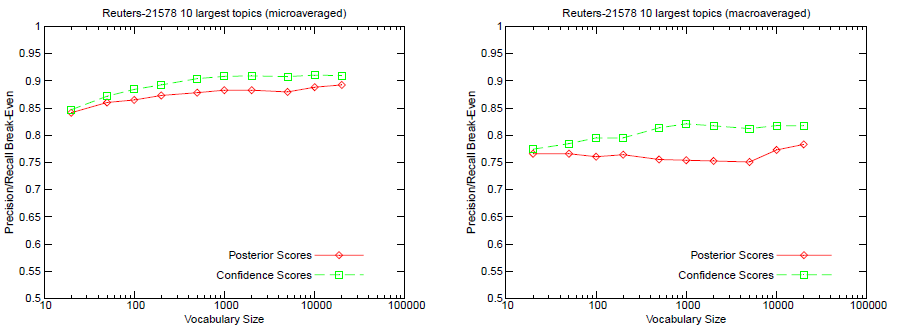
\includegraphics[scale=0.80]{img/klbenefits.png}
\caption{Benefici dell'uso della divergenza di Kullback-Leibler sui corpora REUTERS-21578}
\end{center}
\end{figure}
Inoltre, è importante notare come la misura di confidenza permetta di stabilire di volta in volta se classificare oppure no, infatti possiamo pensare di classificare solo quando il \say{confidence score} di una categoria vada oltre una certa soglia, in certi ambiti questa scelta potrebbe essere fondamentale.
\subsubsection{Approcci ad-hoc}
Oltre agli approcci appena descritti è possibile realizzare degli approcci ad-hoc rispetto a determinati contesti, ad esempio si possono modellare le frequenze tramite la formula TF-IDF:\textit{term frequency-inverse document frequency}\footnotemark
\footnotetext{Raschka, Naive Bayes and Text Classification, Introduction and Theory, 2014}, è un sistema di weighting dei termini, utile quando non si ha un'adeguata stopword-list: 
$$TF-IDF=tf_n(t,d) \cdot idf(t)$$
Dove $tf_n(t,d)$ è la term frequency normalizzata e $idf(t)$ è l'inverse document frequency:
$$ idf(t)=\log{\frac{n_d}{n_d(t)}} $$
Dove $n_d$ è il numero totale dei documenti, e $n_d(t)$ è il numero di documenti che contengono il termine $t$.
\\
\\
Per quanto riguarda le politiche di weighting è possibile pensarle applicate alle parti del documento piuttosto che su tutte le singole feature. Approcci di questo tipo sono ideali quando si hanno degli abstract collegati ai documenti, quando si vogliono valorizzare le feature che occorrono negli abstract o nel titolo dei documenti.
\subsubsection{Performance}
Analisi empiriche comparative ci dicono che il modello multinomiale tende a funzionare meglio del modello di Bernoulli se il vocabolario è relativamente grande.\footnotemark
\footnotetext{McCallum, Nigam, et al, A comparison of event models for naive bayes text classification, in AAAI-98 workshop on learning for text categorization, vol. 752, pp. 41–48, Citeseer, 1998}
\\
\\
Dobbiamo tuttavia considerare che le performance degli algoritmi di machine learning sono altamente dipendenti dalla appropriata scelta delle feature (vedi algoritmi di feature selection). Nella classificazione del testo le performance sono relative anche alla fase di preprocessamento dei corpi testuali: stopword removal, stemming, token-length, n-grammi, lemmatizzazione, disambiguazione, entity recognition. 
\footnotemark
\footnotetext{Rudner, Liang, Automated essay scoring using bayes theorem, The Journal of Technology, Learning and Assessment, vol. 1, no. 2, 2002}
\\
\\
In finale, la scelta tra i vari modelli di classificazione e le tecniche di processamento dei corpi testuali vanno considerate contestualmente al task di classificazione specifico, non esistono soluzioni sempre valide.
\newpage
\section{Algoritmi di feature selection}
La selezione delle feature è una tecnica di riduzione di dimensionalità di feature che fornisce miglior potere predittivo nella modellazione dei dati. È utile quando si lavora con dati di ampie dimensioni oppure quando la raccolta di dati per tutte le feature è proibitiva dal punto di vista dei costi.
\\
\\
La selezione delle feature è, dunque, il processo che ci porta a selezionare un sottoinsieme di feature (termini nella text classification), solo questo sottoinsieme sarà utilizzato come training set per i nostri classificatori. I motivi principali per cui si procede ad una selezione delle feature sono due: innanzi tutto alcuni modelli possono essere addestrati solo con un insieme di feature contenuto, data la loro complessità computazionale in fase di addestramento o predizione. 
\\
\\
In secondo luogo dobbiamo considerare che i classificatori tendono ad essere più precisi quando il numero delle feature è ridotto, molte feature, non solo non sono determinanti nell'individuazione della classe di appartenenza di un documento, ma possono addirittura introdurre un rumore (noise feature). Le \say{noise feature} sono quelle feature che occorrendo accidentalmente in una sola classe si rendono responsabili di errate generalizzazioni che colpiscono l'accuratezza della classificazione (overfitting).
\\
\\
La feature selection talvolta è realizzata in modo totalmente randomica, vale a dire, selezionando sottoinsiemi casuali di feature e validando le performance finché non si raggiungono le prestazioni relative migliori.
\begin{figure}[htbp]
\begin{center}
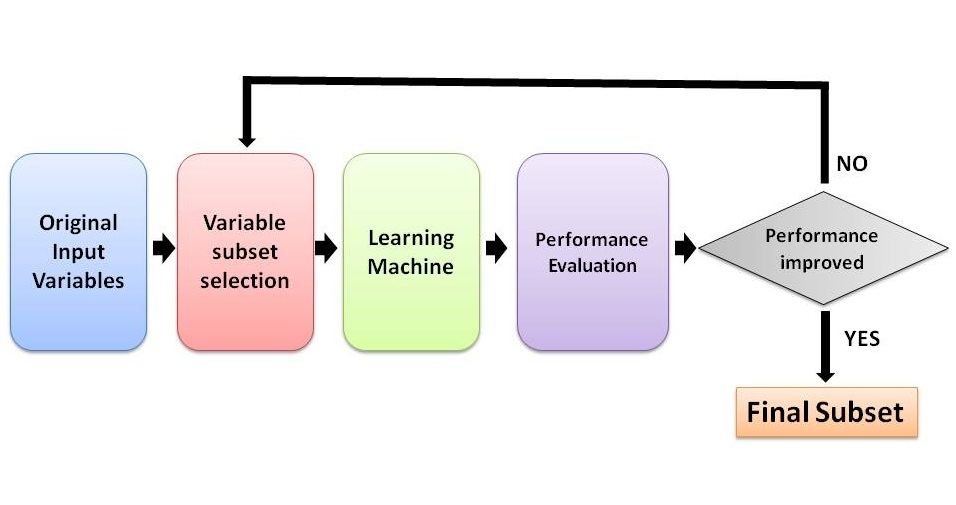
\includegraphics[scale=0.70]{img/fs.jpeg}
\caption{Feature selection randomica}
\end{center}
\end{figure}
Approcci di questo tipo sono molto dispendiosi, solitamente si procede con tecniche più deterministiche basate sulla teoria dell'informazione e della probabilità. Introduction to Information Retrieval\footnotemark descrive tre procedure per la selezione di feature (funzioni di utilità delle feature):
\begin{itemize}  
\item Mutual information
\item Chi square
\item Frequency based
\end{itemize}
\footnotetext{Manning, Raghavan, Schütze, Introduction to Information Retrieval, Cambridge University Press, 2008}
Queste tre procedure forniscono delle metriche per misurare l'utilità di una feature. Indipendentemente dalla misura di utilità che si sceglie, la feature selection seguirà il seguente algoritmo per selezionare le $k$ migliori feature per ciascuna categoria (le più significative):
\\
\\
\begin{verbatim}
SELECT FEATURE(DOCs, CATs, k)
   DOCs: doucumenti
   CATs: classi
   k: numero di top feature da selezionare per classe 
   
   Voc <- EstrazioneVocabolario(DOCs): vocabolario
   L <- []: migliori feature
   U <- []: utilità di tutte le feature   
   
   for each feature t of Voc
         U[t,c]=CalcoloUtilità(t,c)
   
   repeat k times      
      for each categoria c of CATs
         feature t <- Max(U[t,c])       
         L.put(t)
   
   return L
\end{verbatim} 

\newpage
\subsection{Benefici della feature selection}
In \say{Introduction to Information Retrieval (Manning, Raghavan, Schütze)}\footnotetext{Manning, Raghavan, Schütze, Introduction to Information Retrieval, Cambridge University Press, 2008} è presente uno studio sui benefici delle tecniche di feature selection. Il grafico che segue evidenzia i benefici prodotti su alcuni corpora REUTERS, in particolare gli algoritmi di feature selection sono applicati in modo combinato con diversi algoritmi (Naïve Bayes) di classificazione:

\begin{itemize}  
\item Mutual information feature selection - Bayes multinomiale
\item Chi square feature selection - Bayes multinomiale
\item Frequency based feature selection - Bayes multinomiale
\item Mutual information feature selection - Bayes binomiale
\end{itemize}
\begin{figure}[htbp]
\begin{center}
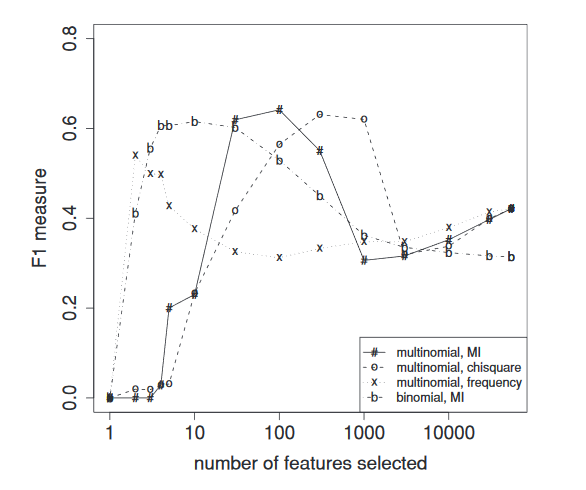
\includegraphics[scale=0.80]{img/fselection.png}
\caption{Benefici della feature selection su alcuni corpora REUTERS}
\end{center}
\end{figure}
Come si può notare, tramite la limitazione del numero di feature si raggiunge una F-measure più alta, in questo caso sia il classificatore multinomiale che quello binomiale è più accurato con circa 100 feature.


\newpage
\subsection{Mutual information feature selection}
Mutual information è una misura di utilità delle feature che sfrutta l'intuizione della teoria dell'informazione. L'informazione mutua di un termine $t$ (feature) e una classe $c$ è la misura di quanto la presenza o assenza della feature contribuisce a determinare la corretta classificazione sulla classe $c$.
\\
\\
Formalmente:
$$I(U,C)=\sum_{e_t \in [0,1]} \sum_{e_c \in [0,1]} P(U=e_t, C=e_c) \log_2 \frac{P(U=e_t, C=e_c)}{P(U=e_t)P(C=e_c)}$$
Dove $U$ è una variabile random che assume il valore $e_t=1$ (il documento contiene il termine $t$), $e_t=0$ (il documento non contiene il termine $t$); analogamente $C$ è una variabile random che assume il valore $e_c=1$ (il documento appartiene alla classe $c$), $e_c=0$ (il documento non appartiene alla classe $c$).
\\
\\
Aritmicamente si ha:
$$I(U,C)=X_{11}+X_{10}+X_{01}+X_{00}$$
$$X{11}=\frac{n_{11}}{n} \cdot \log_2 \frac{n \cdot n_{11}}{(n_{11}+n_{01})\cdot(n_{11}+n_{10})};
X{10}=\frac{n_{10}}{n} \cdot \log_2 \frac{n \cdot n_{10}}{(n_{10}+n_{00})\cdot(n_{11}+n_{10})}$$
$$X{01}=\frac{n_{01}}{n} \cdot \log_2 \frac{n \cdot n_{01}}{(n_{11}+n_{01})\cdot(n_{01}+n_{00})};
X{00}=\frac{n_{00}}{n} \cdot \log_2 \frac{n \cdot n_{00}}{(n_{10}+n_{00})\cdot(n_{01}+n_{00})}$$
\\
\\
con $n$ numero di documenti totali, $n_{tc}$ è il numero di documenti con $e_t \in [0,1]$ e $e_c \in [0,1]$, quindi ad esempio $n_{10}$ è il numero di documenti in cui occorre il termine $t$ ma non la classe $c$, $n_{11}$ è il numero di documenti in cui occorre il termine $t$ e la classe $c$, e così via.
\\
\\
La misura di utilità è, dunque, $I(U,C)$, utilizzando dei valori di soglia per categoria si possono scegliere le $k$ feature più significative per ciascuna categoria.
\subsection{$\chi^2$ feature selection}
Nella selezione delle feature $\chi^2$ si sfrutta l'intuizione probabilistica del test $\chi^2$ che serve a determinare il grado di indipendenza tra eventi, nel nostro caso tra feature e classe di appartenenza:
$$\chi^2(t,c)=\sum_{t \in [0,1]} \sum_{c \in [0,1]} \frac{(N_{e_{t}e_{c}} - E_{e_{t}e_{c}})^2}{E_{e_{t}e_{c}}} $$  
Il calcolo delle $N$ come nel calcolo delle $n$ nell'informazione mutua riguarda le frequenze osservate: $N_{11}$ è il numero di documenti nei quali occorre il termine $t$ nella classe $c$, $N_{10}$ è il numero di documenti nei quali non occorre il termine $t$ nella classe $c$, $N_{01}$ è il numero di documenti nei quali occorre il termine $t$ in tutte le classi eccetto la classe $c$, $N_{00}$ è il numero di documenti nei quali non occorre il termine $t$ in tutte le classi eccetto $c$.
\\ 
\\
Aritmicamente:
$$\chi^2(t,c)=\frac{(n11+n10+n01+n00) \cdot ((n11*n00)-(n10*n01))^2}{(n11+n01)*(n11+n10)*(n10+n00)*(n01+n00)}
$$
$E_{e_{t}e_{c}}$ sono le frequenze attese che il termine $t$ e la classe $c$ occorrano nello stesso documento essendo indipendenti:
$$E_{e_{t}e_{c}} = N \cdot P(t) \cdot P(c)$$
Come si può notare, il calcolo del $\chi^2$ rappresenta lo scarto del valore osservato rispetto all'assunzione di indipendenza delle feature e delle categorie. 
\\
Un alto valore di $\chi^2$ indica che l'ipotesi di indipendenza (la quale indica che il valore atteso ed il osservato devono essere simili) è sbagliata.
\\
\\
I valori di criticità della distribuzione $\chi^2$ con un grado di libertà, ad esempio, se i due eventi sono indipendenti, allora $p$ ($\chi^2>6.63$) è minore di 0.01. Quindi per $\chi^2>6.63$ l'assunzione di indipendenza può essere scartata con una confidenza del 99% 
\\
\\
\begin{tabular}{l*{6}{c}r}
p  & $\chi^2$ critical value \\
\hline
0.1 & 2.71 \\
0.05 & 3.84 \\
0.01 & 6.63 \\
0.005 & 7.88 \\
0.0001 & 10.83 \\

\end{tabular}
\\
\\
Esattamente come l'informazione mutua anche il $\chi^2$ si può considerare misura di utilità della feature, e come per l'informazione mutua è possibile variare il valore di soglia dell'utilità per categoria per selezionare più o meno feature. 
\\
\\
In particolare all'aumentare del valore di $\chi^2$ la probabilità che l'occorrenza della feature e l'occorrenza della categoria siano eventi indipendenti è sempre più bassa (come mostrato nella tabella). Alla luce di questo il valore di soglia dovrà essere molto alto per selezionare poche feature, molto basso per selezionarne di più, e così via.
\subsection{Frequency-based feature selection}
Frequency-based feature selection è la tecnica più intuitiva e più semplice, consiste nell'andare a selezionare solo le feature che occorrono di più nelle varie classi. 
\\
\\
La frequenza può essere considerata come \say{Document frequency} (numero di documenti della classe che contengono una determinata feature), o come \say{Collection frequency} (numero di occorrenze della feature in una classe, senza considerare i documenti).
\say{Document frequency} è più appropriata per il modello di Bernoulli, mentre invece la \say{Collection frequency} è più appropriata per il modello multinomiale. 
\\
\\
Sebbene questo metodo sia molto meno complesso rispetto agli altri due, questo approccio introduce una limitazione, nel selezionare le feature potrebbe includere feature trasversali alle classi, queste feaure non danno un contributo informativo circa il legame tra la feature e la classe.

\newpage
\section{Sperimentazioni e validazione}
La validazione di un sistema di text categorization è basata sulla classificazione di un campione di esempi che sono stati categorizzati manualmente da esperti del dominio. Quando si vuole valutare un sistema di text categorization si devono confrontare le categorie assegnate manualmente con le categorie assegnate dal sistema di text categorization.
\\
\\
Consideriamo la seguente casistica, nella quale diamo una rappresentazione binaria alle varie possibilità di assegnazione di una determinata categoria ad un determinato documento, distinguendo l'assegnazione del sistema da quella dell'esperto del dominio.
\\
\\
\begin{tabular}{l*{6}{c}r}
classe assegnata dall'esperto del dominio:  & SI & NO \\
\hline
classe assegnata dal classificatore: SI & TP & FP \\
classe assegnata dal classificatore: NO & FN & TN \\
\end{tabular}
\\
\\
Abbiamo TP: true positive, FP: false positive, FN: false negative e TN: true negative; questi valori vanno interpretati nel seguente modo:
\begin{itemize}
\item \textbf{true positive:} il sistema e l'esperto del dominio sono coerenti nell'assegnazione della categoria.
\item \textbf{false positive:} la categoria è assegnata dal sistema ma non dall'esperto del dominio.
\item  \textbf{true negative:} la categoria non è assegnata né dal sistema né dall'esperto del dominio.
\item \textbf{false negative:} la categoria è assegnata dall'esperto ma non dal sistema.
\end{itemize}


\subsection{Metriche per l'evaluation}
Piuttosto che avere tutti questi valori binari per ciascuna coppia documento-categoria siamo interessati ad avere quattro valori che rappresentino ciascuna delle quattro tipologie (true positive, false positive, true negative, false negative), pertanto è necessario sommare questi quattro valori per tutte le coppie documento-categoria. Questi quattro valori sono le grandezze che stanno alla base di varie metriche utili per l'evaluation del sistema di classificazione.

\[ Precision: \quad P= \frac{TP}{TP+FP} \]
\\
La Precision è una misura utile per quantificare la precisione del sistema sul campione di categorie selezionate a valle della classificazione, è il rapporto tra le categorie correttamente assegnate e tutte quelle assegnate.
\[ Recall: \quad R= \frac{TP}{TP+FN} \]
La Recall (in italiano \say{recupero}) è utile per misurare la frazione di categorie assegnate dall'esperto a valle della classificazione del sistema. La recall è il rapporto tra categorie assegnate e tutte le categorie di appartenenza di un documento. 
\\
Recall e Precision sono due metriche basilari nei sistemi di information retrieval, trovare un equilibrio tra queste due grandezze non è facile, è necessario un compromesso, in quanto, incrementando la precision abbiamo il declino della recall e viceversa. In una categorizzazione multi-label nella quale restituiamo poche categorie per documento è verosimile avere precision alta e recall bassa, mentre invece, se assegniamo molte categorie sarà più probabile avere recall alta a scapito di precision.


\[ Fallout: \quad F= \frac{FP}{FP+TN} \]

\[ Accuracy: \quad F= \frac{TP+TN}{TP+FP+FN+TN} \]
Utile per quantificare l'accuratezza generale del sistema.
\[ Error: \quad F= \frac{FP+FN}{TP+FP+FN+TN} \]
F-measure e Interpolated-break-even sono due grandezze che sintetizzano in un solo valore la precision e la recall di un sistema di classificazione:
\\
La F-measure (anche nota come F1-score) è la media armonica 
\[ F-measure: \quad F1= \frac{2PR}{P+R} \]
\[ Interpolated-break-even: \quad IB= \frac{P+R}{2} \]

Tra le due metriche è preferibile usare l'F1, in quanto più sensibile a valori di precision o recall molto bassi.

\subsection{K-fold-cross-validation}
Gli algoritmi di apprendimento supervisionati per la categorizzazione dei testi (Bayesiani, margin-based, vettoriale, ...) hanno bisogno di un test-set ed un training-set per poter essere valutati. Questi due insiemi devono essere disgiunti per avere delle buone stime delle performance del sistema di classificazione.
\\
Training set: è un insieme di esempi usato per l'addestramento (apprendimento) del classificatore.
\\
\\
Validation set: è un insieme di esempi usato per regolare i parametri del classificatore.
\\
\\
Test set: è uni insieme di esempi usato per assegnare le performance di un classificatore addestrato.
\\
\\
Se non separassimo gli insiemi di test e di validation la stima di errore di un modello sulla validazione sarà parziale (inferiore) in quanto il validation set è utilizzato per selezionare il modello finale, infine si può procedere alla valutazione del modello finale sul test set.
\footnotetext{Gutierrez-Osuna, Introduction to Pattern Analysis, Texas A\&M University}
\\
\\
La k-fold-cross-validation (in italiano validazione incrociata) è una tecnica utilizzabile in presenza di un training set abbastanza grande. In particolare la k-fold cross-validation consiste nella suddivisione del dataset totale in k parti di uguale numerosità e, ad ogni passo, la k-esima parte del dataset viene ad essere il test dataset, mentre la restante parte costituisce il training dataset.
\\
\\
Così, per ognuna delle k parti (di solito k=10, k=5) si allena il modello, evitando quindi problemi di overfitting, ma anche di campionamento asimmetrico (e quindi affetto da bias) del training dataset, tipico della suddivisione del dataset in due sole parti (ovvero training e test dataset). In altre parole, si suddivide il campione osservato in gruppi di uguale numerosità, si esclude iterativamente un gruppo alla volta e lo si cerca di predire con i gruppi non esclusi. Ciò al fine di verificare la bontà del modello di predizione utilizzato.

\newpage
\section{Sistemi di catalogazione}
I sistemi di categorizzazione dei testi coprono differenti aeree di interesse. I sistemi di categorizzazione sono stati realizzati per rispondere alla necessità di catalogare ed indicizzare i documenti. 
\\
I task di categorizzazione multi label sono molto complessi ed i risultati ottenuti spesso sono molto distanti dai livelli accettabili di accuratezza.
\\
\\
Molti approcci sono stati esplorati ed implementati, tra questi abbiamo i sistemi keyword-based (come MeSH, BIOSIS, e NASA MAI System), i quali sono stati pensati per la realizzazione di abstract, vale a dire l'individuazione di keyword (tag) che diano una descrizione semantica, sintetica ed univoca (standard) del contenuto dei documenti. 
\\
\\
Un'altra classe di algoritmi utilizzati per la catalogazione multi label dei testi è quella basata su tecniche di machine learning, come ad esempio possono essere gli algoritmi margin-based (SVM), tecniche bayesiane, modelli a spazi vettoriali (VSM). Il classificatore EuroVoc JRC-JEX è basato su particolare approccio VSM.
\\
\\
Segue una descrizione in astratto dei sistemi MeSH, BIOSIS, NASA MAI System, e JRC-JEX; con un particolare focus su quest'ultimo essendo l'indexer più vicino al task di classificazione open-data.
\subsection{JRC-JEX (JRC EuroVoc Indexer)}
Il classificatore JEX, sviluppato presso i laboratori JRC (Joint Research Centre) è stato presentato nell'ambito del workshop \say{Ontologies and Information Extraction at EUROLAN 2003: The Semantic Web and Language Technology – Its Potential and Practicalities}. 
\\
\\
JEX è un classificatore multi-label, addestrato con il corpus JRC-Acquis (training set) categorizza con i descrittori (concetti) del tesauro EuroVoc con tecniche basate sull'approccio \say{VSM} (vector space model).
La scelta di basare il classificatore su EuroVoc e JRC-Acquis rende il sistema multilingua e garantisce la copertura di tutte le tematiche di interesse della politica europea. 
\\
\\
Sul sito di JEX si descrivono in sintesi le funzionalità di questo sistema:
\\
\textit{\say{Multilingual Eurovoc thesaurus descriptors are used by a large number of European Parliaments and Documentation Centres to manually index their large document collections. The assigned descriptors are then used to search and retrieve documents in the collection and to summarise the document contents for the users. 
\\
\\
As Eurovoc descriptors exist in one-to-one translations in almost thirty languages, they can be displayed in a language other than the text language and give users cross-lingual access to the information contained in each document. At the same time, EuroVoc is an ideal means to search in the user's language and to retrieve documents in other languages.
\\
\\
The European Commission's (EC) Joint Research Centre (JRC) has developed - and makes available - software that automatically assigns EuroVoc descriptors to documents in currently 22 languages. The system uses statistical Machine Learning methods that learn the multi-label categorisation rules from previously manually indexed documents. The method used can be described as profile-based category ranking. 
\\
\\
This software, called JRC EuroVoc Indexer, or short JEX, has been trained for 22 languages and is available for download from this site. The software allows users to re-train the software on their own data, even using their own, alternative classification systems}}
\\
\\
La decisione di rilasciare gratuitamente JEX è in linea con la Direttiva 2003/98/EC del parlamento europeo sul riuso delle informazioni delle pubbliche amministrazioni europee, la Direttiva riconosce l'importanza strategica della pubblicazione di collezioni di documenti multilingua al fine di migliorare prodotti e servizi \say{cross-border}. In questa prospettiva è stato rilasciato anche JRC-Acquis parallel corpus (Steinberg et al. 2006), il DGT-TM translation memory (Steinberg et al. 2012), e JRC-Names (Steinberg et al. 2011) che è un sistema per la named entity recognition.
\subsubsection{Pre-processamento corpus}
Al fine di realizzare un sistema di catalogazione multilingua, la fase di elaborazione dei corpus (corpus pre-processing) è stata implementata con tecniche elementari (indipendenti dalla lingua). In realtà inizialmente si pensava fosse fondamentale l'utilizzo di feature multi-word (ad esempio \say{green plant} vs \say{power plant}), o lemmatizzate per favorire notevolmente l'accuratezza oltre alla classica \say{stop-word list}; specialmente per alcune lingue con forme di coniugazione più complesse di quelle inglesi come lo spagnolo, il francese e l'italiano. 
\begin{figure}[htbp]
\begin{center}
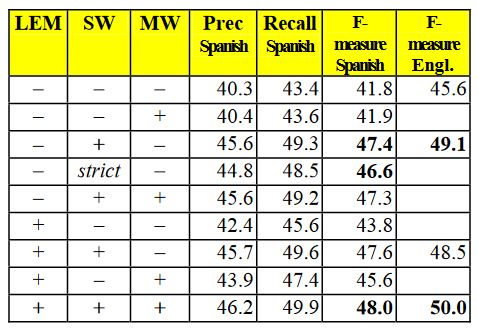
\includegraphics[scale=1.00]{img/jexfmeasure.png}
\caption{F-measure al variare delle tecniche di pre-processamento dei corpus}
\end{center}
\end{figure}
\\
\\
Sebbene queste tecniche migliorino la F-measure di JEX, i risultati ottenuti utilizzando solamente una buona \say{stop-word list} sono circa uguali sia per la lingua spagnola che per la lingua inglese (Spagnolo F-measure = 47.4 vs 48).
\\
\\
L'utilizzo di una buona \say{stop-word list} porta dei benefici (Spagnolo F-measure = 46.6 vs 47.4), questa situazione è particolarmente vantaggiosa per la realizzazione di un sistema di catalogazione multilingua, utilizzando solamente delle \say{stop-word list} si è sostanzialmente disaccoppiati dalla lingua in cui si classifica.
\footnotemark
\footnotetext{Pouliquen, Steinberger, Ignat, Automatic Annotation of Multilingual Text Collections with a Conceptual Thesaurus, JRC, 2003}  
\subsubsection{Vector space model}
L'algoritmo di classificazione sul quale è basato JEX è un adattamento di una tecnica di information retrieval al problema della categorizzazione dei testi: il modello a spazi vettoriali. 
\\
\\
\textit{
Vector space model or term vector model is an algebraic model for representing text documents (and any objects, in general) as vectors of identifiers, such as, for example, index terms. It is used in information filtering, information retrieval, indexing and relevancy rankings. (wikipedia-eng)
}
\\
\\
Vector Space Model (VSM) sfrutta un'intuizione geometrica nella rappresentazione dei documenti, ogni documento è un vettore le cui componenti sono i termini che lo compongono e il valore assunto dalle componenti può essere associato a diverse misure: term frequency, term frequency normalizzata, tf-idf, document frequency, chi-square, log-likelihood.
\\
\\  
VSM nella categorizzazione dei testi è essenzialmente applicata seguendo due tecniche: k-nearest-neighbor (kNN) e Rocchio.\footnotemark
\footnotetext{Manning, Raghavan, Schütze, Introduction to Information Retrieval, Cambridge University Press, pp. 289-290, 2008}
\\
\\
La classificazione VSM-Rocchio divide lo spazio vettoriale in regioni in base ai centroidi (\say{prototypes}), uno per ogni categoria (concetti EuroVoc nel caso di JEX), questi centroidi o prototipi sono i centri di massa (baricentri) di tutti i vettori di una determinata categoria. La classificazione VSM-Rocchio è semplice e efficiente ma inaccurata in alcuni casi, ad esempio quando la distribuzione dei documenti per categoria non è esattamente rappresentabile come una sfera nello spazio vettoriale
\\
\\
La classificazione VSM-kNN assegna la categoria dei k vettori più vicini al vettore del documento che va classificato. kNN non richiede necessariamente una fase di addestramento. Sebbene sia più preciso del metodo Rocchio, questo metodo è sostanzialmente più pesante dal punto di vista computazionale perché si devono confrontare tutti i documenti dello spazio vettoriale con il vettore del documento da classificare. Generalmente training set grandi hanno una distribuzione delle categorie non completamente uniformi e sferiche, in questi casi VSM-kNN classificherà meglio rispetto al metodo Rocchio.
\\
\\
L'approccio adottato da JEX è un approccio VSM-Rocchio nel quale la selezione dei termini (componenti dei vettori) è basata sulla metrica log-likelihood descritta da Kligarriff (1996).\footnotemark In JEX il valore assunto dal log-likelihood dai termini (o lemmi) serve a determinare la \say{lista degli associati}, che sono le componenti dello spazio vettoriale, pertanto questa metrica serve a realizzare la feature selection.
\footnotetext{Kilgarriff, Which words are particularly  
characteristic of a text? A survey of statistical approaches. Proceedings of the AISB Workshop on Language Engineering for Document Analysis and Recognition, pp. 33-40, 1996}

\subsubsection{Weighting dei vettori}
Al fine di determinare il peso di un associato (associato = feature = lemma = termine) per un descrittore (descrittore = concetto = categoria) JEX non utilizza la metrica log-likelihood ma una variazione della formula TF-IDF nella quale si considera la descriptor-frequency piuttosto che la document-frequency. Esattamente come nella formula TF-IDF si vogliono penalizzare i termini che occorrono in tanti descrittori diversi (piuttosto che documenti diversi).
\\
La formula per stabilire il peso delle feature (componenti dei vettori nello spazio vettoriale) è $Weight_{l,d}$ (per il lemma $l$ e il descrittore $d$):
\\
\[Weight_{l,d}=W_{l,d} \cdot IDF_l \]
\\
$W_{l,d}$ è il peso di un lemma relativamente ad un descrittore, mentre $IDF_l$ è l'\say{Inverse Descriptor Frequency}.
\\
\[W_{l,d}=\sum_{t \in T_{l,d}} \frac{1}{Nd_t} \]
\\
$Nd_t$ è il numero di descrittori manualmente assegnati al documento $t$, $T_{l,d}$ sono i documenti che contengono il lemma $l$ e il descrittore $d$. La normalizzazione rispetto la lunghezza dei documenti non fornisce buoni risultati, mentre invece si è visto che la normalizzazione rispetto al numero di descrittori è una buona scelta soprattutto per diminuire l'interferenza tra i descrittori.
\\
\[IDF_{l}= log \Bigg(\frac{Max_{DF_{l}}}{\beta \cdot DF_l}+1 \Bigg) \]
\\
$DF_l$ è il numero di descrittori nei quali il lemma compare come associato, mentre invece $Max_{DF_{l}}$ è il massimo valore di $DF$ per tutti i lemmi.
\\
Il parametro $\beta$ è settato a 10 al fine di penalizzare i lemmi che occorrono di più del 10\% di $Max_{DF_{l}}$.
\\
In finale otteniamo la formula:
\\
\[Weight_{l,d}=\sum_{t \in T_{l,d}} \frac{1}{Nd_t} \cdot log \Bigg(\frac{Max_{DF_{l}}}{\beta \cdot DF_l}+1 \Bigg) \]
\\
Sono state provate le seguenti misure di similarità tra il vettore del documento da classificare ed i vettori che rappresentano i descrittori:
\begin{itemize}
\item \textbf{Cosine formula:} (Salton, 1989)\footnotemark\footnotetext{Salton, Automatic Text Processing: the Transformation, Analysis and Retrieval of Information by Computer, Addison-Wesley, 1989}
\item \textbf{Okapi formula:} (Robertson et al., 1994)\footnotemark
\item  \textbf{Prodotto scalare:} Cosine formula senza normalizzazione
\item \textbf{Una combinazione lineare delle formule Cosine, Okapi e prodotto scalare:} (Wilkinson, 1994)
\end{itemize}
La combinazione lineare delle formule di similarità è una soluzione molto buona, i coefficienti di proporzionalità vanno assegnati in base alla lingua e in base ad altri parametri, tuttavia si è visto che la proporzione 40\%-20\%-40\% è la migliore in molti casi.

\footnotetext{Robertson, Walker, Hancock-Beaulieu, Gatford, Okapi in TREC-3. Proceedings of Text Retrieval Conference  TREC-3, U.S. National Institute of Standards and Technology,   
Gaithersburg, USA. NIST Special Publication 500-225, pp. 109-126, 1994}

\newpage
\subsection{BIOSIS}
Uno dei più sofisticati programmi per l'indicizzazione automatica sviluppato negli studi BIOSIS è stato discusso da  Vleduts-Stokolov; \footnotetext{Vleduts-Stokolov, Concept recognition in an automatic text-processing system for the life sciences, 1987} le parole che occorrono nei titoli delle pubblicazioni che sono anche contenute all'interno di un vocabolario semantico. Il quale vocabolario semantico rappresenta la terminologia scientifica rappresentata da circa 15'000 termini.
I termini coprono i seguenti campi di studio: agricoltura, anatomia, comportamento, biochimica, bioingegneria, biofisica, biotecnologie, botanica, biologia cellulare, biologia ambientale, medicina clinica sperimentale, genetica, immunologia, microbiologia, patologia, farmacologia, fisiologia e tossicologia.
\\
\\
\url{www.cas.org/File%20Library/Training/STN/DBSS/biosis.pdf}
\\
\\
Questi 15'000 termini sono mappati su un vocabolario di 600 concetti (Concept Headings), pertanto un Concept Heading può essere assegnato dal sistema sulla base della presenza o meno di alcuni termini nei titolo. Vleduts-Stokolov ha documentato l'accuratezza di BIOSIS, notando che il sistema si comporta come un umano nella assegnazione dei concetti del vocabolario nel 61\% dei casi. Al fine di rendere più accurato il sistema si è pensato di utilizzare più livelli di astrazione dei concetti che stanno al di sopra dei termini (primario, secondario e terziario), portando così l'accuratezza al 75\%.

\subsection{NASA MAI System}
Nasa Center for Aerospace Information (CASI) ha un database contenente tre milioni di record, almeno due milioni sono report tecnici e articoli di giornale. La CASI indicizza i documenti al fine di ottenere degli abstract. Nasa MAI System (MAI è acronimo di Machine Aided Indexing) è un sistema di sostegno utilizzato dagli utenti (specialisti del dominio) per navigare e selezionare un'insieme di possibili parole chiave da utilizzare per annotare i documenti.
Questo sistema è stato pensato per produrre delle annotazioni più coerenti, in quanto l'esperto del dominio è guidato dalle connessioni tra i concetti di un vocabolario. 
\\
\\
Il progetto NASA MAI è stato pensato per minimizzare lo sforzo per la re-indicizzazione di documenti già indicizzati da altre agenzie, infatti, quando il progetto è iniziato circa la metà dei report tecnici all'interno del NASA STI (database) erano stati indicizzati da agenzie diverse.  
Questi report, ricevuti in forma machine-readable, sono convertiti utilizzando tecniche di processamento del linguaggio naturale.
\\
\\
Lo scopo principale di NASA MAI System è quello di fornire un'insieme di termini \say{adeguati} per l'annotazione dei documenti. Molti documenti provenienti da altre agenzie utilizzavano dei termini non corrispondenti al vocabolario utilizzato dalla NASA. L'utilizzo di un unico vocabolario specializzato permette di collegare i concetti a vari livelli di astrazione, e sfruttare i sinonimi nella ricerca dei documenti. Per ogni termine, MAI, propone una serie di termini candidati corrispondenti ai \say{NASA terms}.  
\\
\\
Il NASA MAI System non è basato su sofisticate tecniche di processamento del linguaggio naturale e parsing grammaticale, segue un approccio rule-based che approssima i risultati dei parsing più approfonditi, e, che richiedono un notevole sforzo computazionale. Le regole sono sviluppate al fine di ottenere dei termini (feature testuali) che meglio rappresentino i concetti.
\\
\\
MAI usa una grande knowledge base (manutenuta), oltre 170'000 termini e frasi, oltre alle regole. I valori di precision e recall sono attorno al 50\% (break-even point), sebbene possa sembrare basso questo risultato è piuttosto buono se si considera la vastità di argomenti coperti e la diversità dei documenti processati.

\subsection{MeSH}
MeSh (acronimo di Medical Subject Headings), è un indicizzatore automatico utilizzato dalla U.S National Library of Medicine, il quale utilizza un database di circa 18'000 termini del campo medico. Le tecniche adottate sono simili a quelle già descritte negli altri indexer keyword-based.
\url{https://www.nlm.nih.gov/pubs/factsheets/mesh.html}


\newpage
\section{Aspetti software}
\subsection{Architettura}
\subsection{Deployment}

\newpage
\section{Bibliografia e risorse}
\subsection{Bibliografia}
\begin{itemize}
\item Di Noia, De Virgilio, Di Sciascio, Donini, Semantic Web: Tra ontologie e Open Data, Apogeo, 2013
\item Linee guida per i siti web della pubblica amministrazione, articolo 4 Direttiva 8/09, Ministero della pubblica amministrazione
\item Steinberger, Ebrahim, Poulis, Carrasco-Benitez, Schlüter, Przybyszewski \& Gilbro. An overview of the European Union's highly multilingual parallel corpora. Language Resources and Evaluation Journal, JRC, 2014
\item Steinberger, Ebrahim, Turchi. JRC EuroVoc Indexer JEX - A freely available multi-label categorisation tool. European Commission, JRC, 2014
\item Profilo italiano di DCAT-AP (DCAT Application Profile for data portals in Europe), Versione 1.0, Agenzia per l'Italia digitale, 2006
\item Busa, Fondamenti di informatica linguistica, Istituto Geografico De Agostini, 1987
\item Chiari, Introduzione alla linguistica computazionale, Laterza, 2007
\item Orsingher, Beghin, Introduzione alla probabilità, Carocci editore
\item Porter, An algorithm for suffix stripping, Program: electronic library and information systems, vol. 14, no. 3, pp. 130–137, 1980
\item Mitchell, Machine learning, Mc Graw Hill, 1997
\item Shimodaira, Text classification using Naive Bayes, 2015
\item Raschka, Naive Bayes and Text Classification, Introduction and Theory, 2014
\item Rudner, Liang, Automated essay scoring using bayes theorem, The Journal of Technology, Learning and Assessment, vol. 1, no. 2, 2002
\item McCallum, Nigam, et al, A comparison of event models for naive bayes text classification, in AAAI-98 workshop on learning for text categorization, vol. 752, pp. 41–48, Citeseer, 1998
\item Domingos, Pazzani, On the optimality of the simple bayesian classifier under zero-one loss, Machine learning, vol. 29, no. 2-3, pp. 103–130, 1997
\item Zhang, The optimality of naive bayes, AA, vol. 1, no. 2, p. 3, 2004
\item Manning, Raghavan, Schütze, Introduction to Information Retrieval, Cambridge University Press, 2008
\item Schneider, Techniques for Improving the Performance of Naive Bayes for Text Classification, University of Passau, Department of General Linguistics
\item Craven, Di Pasquo, Freitag, McCallum, Mitchell, Nigam, Slattery, Learning to construct knowledgebases from the World Wide Web. Artificial Intelligence 118, pp. 69-113, 2000
\item Gutierrez-Osuna, Introduction to Pattern Analysis, Texas A\&M University
\item Pouliquen, Steinberger, Ignat, Automatic Annotation of Multilingual Text Collections with a Conceptual Thesaurus, JRC, 2003
\item Kilgarriff, Which words are particularly  
characteristic of a text? A survey of statistical approaches. Proceedings of the AISB Workshop on Language Engineering for Document Analysis and Recognition, pp. 33-40, 1996
\item Salton, Automatic Text Processing: the Transformation, Analysis and Retrieval of Information by Computer, Addison-Wesley, 1989
\item Robertson, Walker, Hancock-Beaulieu, Gatford, Okapi in TREC-3. Proceedings of Text Retrieval Conference  TREC-3, U.S. National Institute of Standards and Technology,   
Gaithersburg, USA. NIST Special Publication 500-225, pp. 109-126, 1994
\item Vleduts-Stokolov, Concept recognition in an automatic text-processing system for the life sciences, 1987
\item Fumagalli, Trasparenza e Open Data: l'evoluzione del quadro normativo fino all'emanazione del neo D.Lgs. 33/2013. La Bussola della Trasparenza, 2014
\end{itemize}

\newpage
\subsection{Link utili}
\begin{itemize}
\item \url{https://github.com/simonegasperoni/open-cata}
\item \url{http://opendefinition.org/od/2.1/en}
\item \url{http://opendatahandbook.org/guide/it/what-is-open-data}
\item \url{http://dati.mit.gov.it/dcat/catalog.rdf}
\item \url{https://www.w3.org/TR/vocab-dcat}
\item \url{https://ckan.org}
\item \url{https://github.com/ckan/ckan}
\item \url{https://datahub.io}
\item \url{https://europeandataportal.eu}
\item \url{http://sciamlab.com/opendatahub/it}
\item \url{http://dati.gov.it}
\item \url{https://github.com/ckan/ckanext-dcat}
\item \url{https://github.com/ckan/ckanext-dcat#rdf-dcat-to-ckan-dataset-mapping}
\item \url{http://eurovoc.europa.eu}
\item \url{https://ec.europa.eu/jrc/en/language-technologies/jrc-acquis}
\item \url{https://ec.europa.eu/jrc/en/language-technologies/jrc-eurovoc-indexer}
\item \url{http://tei-c.org}
\item \url{http://snowballstem.org}
\item \url{https://github.com/snowballstem/snowball}
\item \url{https://www.nlm.nih.gov/pubs/factsheets/mesh.html}
\item \url{www.cas.org/File%20Library/Training/STN/DBSS/biosis.pdf}
\end{itemize}

\newpage
\section{Appendice}

\subsection{Qualità dei dataset secondo il W3C}
Per distinguere i diversi formati utilizzabili nella codifica dei set di dati o dataset (insieme di dati pubblicati), è stato proposto in seno al W3C (World Wide Web Consortium, un Consorzio internazionale fondato nel 1994 con l'obiettivo di potenziare e diffondere il WWW) dal suo Presidente ed ideatore, Tim Berners-Lee, un modello di catalogazione che li classifica in base alle loro caratteristiche su una scala di valori da 1 (una stella) a 5 (cinque stelle):
\\
\begin{itemize}
\item \textbf{1 stella:} Dati grezzi. Sono dati raccolti che non sono stati soggetti a nessun processo, aggregazione o manipolazione, che sono disponibili in quei formati che – seppure disponibili su supporto informatico – non consentono un'estrapolazione immediata degli stessi. Rappresentano, cioè, il livello base costituito da file non strutturati: ad esempio immagini nei diversi formati grafici bitmap (.gif, .Jpg, .bmp, .png, ecc…), documenti in formato Microsoft Word, file in formato Adobe Pdf. Una sola stella indica la semplice disponibilità di un'informazione e di un dato on line, in un formato qualsiasi, purché distribuito con licenza aperta. I dati distribuiti in questo formato sono leggibili e stampabili dagli utenti, possono essere conservati localmente su un PC e sono semplici da pubblicare. Tuttavia non sono un formato aperto in quanto non è possibile effettuare su di essi alcuna elaborazione.

\item \textbf{2 stelle:} Dati strutturati. Questo livello indica dati strutturati ma codificati con un formato proprietario (ad esempio documenti realizzati con fogli di calcolo come Microsoft Excel salvati in formato .xls, ecc…). Due stelle indicano, oltre alle possibilità offerte dai dati contraddistinti da una sola stella, la possibilità di effettuare elaborazioni e sistematizzazioni in forma strutturata sui dati, a patto di disporre del software necessario a gestire un file codificato con un formato proprietario. I dati caratterizzati dalle due stelle non sono un formato aperto in quanto per elaborarli è necessario un software proprietario, tuttavia di norma possono essere convertiti – essendo dati strutturati – in dati aperti.

\item \textbf{3 stelle:} Dati strutturati. Questo livello indica dati strutturati e codificati in un formato non proprietario. Ad esempio documenti realizzati con fogli di calcolo come OpenOffice Calc salvati in formati come .csv (Comma Separated Values), .sxc, al posto – ad esempio – del formato Microsoft Excel. Tre stelle indicano, oltre alle possibilità offerte dai dati contraddistinti da due sole stelle, la possibilità di effettuare elaborazioni e sistematizzazioni in forma strutturata sui dati senza essere costretti ad utilizzare software proprietario. Quello caratterizzato dalle tre stelle è il formato più semplice di dati aperti.

\item \textbf{4 stelle:} Dati presenti in database. Questo livello indica dati strutturati e codificati in un formato non proprietario che sono dotati di un URI (Uniform Resource Identifier – Identificatore Univoco di Risorsa, ossia di norma un indirizzo internet nel formato http://www.nomedominio.it/) che li rende indirizzabili sulla rete e quindi utilizzabili direttamente on line attraverso l'inclusione in una struttura basata sul modello RDF (Resource Description Framework). Quattro stelle indicano quindi il fatto che il singolo dato di un dataset, disponibile on line in un formato aperto (tipicamente XML/RDF) può essere richiamato attraverso un URL (Uniform Resource Locator, indirizzo Web che identifica univocamente una risorsa su internet ed è la tipologia più frequente e riconosciuta di URI) specifico. Ciò consente di puntare al dato o ad un insieme di dati da una applicazione o accedervi dall'interno di un programma che può poi elaborarlo in vari modi.

\item \textbf{5 stelle:} Dati presenti in database. Questo livello indica quelli che vengono definiti Linked Open Data (LOD), dati aperti, cioè, che – dal punto di vista del formato – oltre a rispondere alle caratteristiche della classificazione a quattro stelle presentano anche, nella struttura del dataset, collegamenti ad altri dataset. In altri termini, grazie al ricorso al modello di descrizione dei dati RDF, è possibile collegare dinamicamente tra loro più dataset, incrociando così informazioni provenienti da fonti diverse, eventualmente gestite da diverse Amministrazioni.
\end{itemize}
\phantom
\\
\footnotetext{Fumagalli, Trasparenza e Open Data: l'evoluzione del quadro normativo fino all'emanazione del neo D.Lgs. 33/2013. La Bussola della Trasparenza, 2014}

\newpage
\subsection{Associazione Temi DCAT - Microtesauri EuroVoc}
Microtesauri EuroVoc associati al tema DCAT-AP (EU Data Themes): AGRI (Agriculture, Fisheries, Forestry \& Foods) 
\begin{verbatim}
    5606 agricultural policy
    5611 agricultural structures and production 
    5616 farming systems 
   	5621 cultivation of agricultural land 
   	5626 means of agricultural production 
   	5631 agricultural activity
   	5636 forestry 
   	5641 fisheries
   	6006 plant product
   	6011 animal product 
   	6021 beverages and sugar beverage sugar 
   	6026 foodstuff 
   	6031 agri-foodstuffs
   	6036 food technology
\end{verbatim}
Microtesauri EuroVoc associati al tema DCAT-AP (EU Data Themes): ENER (Energy) 
\begin{verbatim}
    6606 energy policy 
    6616 oil industry 
    6621 electrical and nuclear industries 
    6626 soft energy
    6611 coal and mining industries
\end{verbatim}
Microtesauri EuroVoc associati al tema DCAT-AP (EU Data Themes): REGI (Regions \& Cities) 
\begin{verbatim}
    7206 Europe
    7211 regions of EU Member States 
    7216 America 
    7221 Africa
    7226 Asia and Oceania
    7231 economic geography 
    7236 political geography
    7241 overseas countries and territories
\end{verbatim}
Microtesauri EuroVoc associati al tema DCAT-AP (EU Data Themes): TRAN (Transport)
\begin{verbatim}
    4806 transport policy
    4811 organisation of transport 
    4816 land transport land transport 
    4821 maritime and inland waterway transport 
    4826 air and space transport
\end{verbatim}
Microtesauri EuroVoc associati al tema DCAT-AP (EU Data Themes): ECON (Economy \& Finance) 
\begin{verbatim}
    1606 economic policy 
    1611 economic growth 
    1616 regions and regional policy 
    1621 economic structure 
    1626 national accounts 
    1631 economic analysis 
    2406 monetary relations
    2411 monetary economics
    2416 financial institutions and credit
    2421 free movement of capital
    2426 financing and investment 
    2431 insurance
    2436 public finance and budget policy 
    2441 budget 
    2446 taxation
    2451 prices
    2006 trade policy
    2011 tariff policy 
    2016 trade supply
    2021 international trade 
    2026 consumption 
    2031 marketing
    4006 business organisation
    4011 business classification
    4016 legal form of organisations
    4021 management
    4026 accounting
    4031 competition 
    6806 industrial structures
    6811 chemistry 
    6816 iron
    6821 mechanical engineering
    6826 electronics and electrical engineering
    6831 building and public works
    6841 leather and textile industries 
    6846 miscellaneous industries 
\end{verbatim}
Microtesauri EuroVoc associati al tema DCAT-AP (EU Data Themes): INTR (International Issues) 
\begin{verbatim}
    7606 United Nations
    7611 European organisations 
    7616 extra-European organisations 
    7621 world organisations
    7626 non-governmental organisations
    0811 cooperation policy
    0816 international balance 
    0821 defence 
\end{verbatim}
Microtesauri EuroVoc associati al tema DCAT-AP (EU Data Themes): GOVE (Government \& Public Sector) 
\begin{verbatim}
    0406 political framework
    0411 political party 
    0416 electoral procedure and voting election
    0421 parliament 
    0426 parliamentary proceedings
    0431 politics and public safety 
    0436 executive power and public service 
    1006 Community institutions and European civil service 
    1011 European Union law 
    1016 European construction
\end{verbatim}
Microtesauri EuroVoc associati al tema DCAT-AP (EU Data Themes): JUST (Justice, Legal System \& Public Safety) 
\begin{verbatim}
    1206 sources and branches of the law 
    1211 civil law 
    1216 criminal law 
    1221 justice access to the courts 
    1226 organisation of the legal system 
    1236 rights and freedoms
\end{verbatim}
Microtesauri EuroVoc associati al tema DCAT-AP (EU Data Themes): ENVI (Environment) 
\begin{verbatim}
    5206 environmental policy
    5211 natural environment
    5216 deterioration of the environment 
\end{verbatim}
Microtesauri EuroVoc associati al tema DCAT-AP (EU Data Themes): EDUC (Education, Culture \& Sport) 
\begin{verbatim}
    3206 education
    3211 teaching 
    3216 organisation of teaching 
    3221 documentation 
    3226 communications
    3231 information and information processing
    3236 information technology and data processing 
    2831 culture and religion arts cultural policy culture
\end{verbatim}
Microtesauri EuroVoc associati al tema DCAT-AP (EU Data Themes): HEAL (Health) 
\begin{verbatim}
    2841 health
\end{verbatim}
Microtesauri EuroVoc associati al tema DCAT-AP (EU Data Themes): SOCI (Population \& Society) 
\begin{verbatim}
    2806 family 
    2811 migration internal 
    2816 demography and population composition 
    2821 social framework
    2826 social affairs
    2836 social protection
    2846 construction and town planning 
    4406 employment
    4411 labour market 
    4416 organisation of work and working conditions 
    4421 personnel management and staff remuneration
    4426 labour law and labour relations
\end{verbatim}
Microtesauri EuroVoc associati al tema DCAT-AP (EU Data Themes): TECH (Science \& Technology)
\begin{verbatim}
    3606 natural and applied sciences 
    3611 humanities behavioural 
    6406 production 
    6411 technology and technical regulations
\end{verbatim}

\end{document}
